% ---------- Packages ----------
% Document Settings
\documentclass[12pt]{report}
\usepackage[toc,page]{appendix}
\usepackage[a4paper,left=40mm,top=25mm,bottom=25mm,right=40mm]{geometry}
\usepackage[utf8]{inputenc}
\linespread{1.25}

% Text
\usepackage{hyperref}
\usepackage{color}

% Images
\usepackage{caption}
\usepackage{graphicx}
\usepackage{subcaption}
\usepackage{wrapfig}

% Tables
\usepackage{booktabs}
\usepackage{array}
\usepackage{multirow}
\usepackage{booktabs}
\usepackage{float}

% Headers and Footers
\usepackage{fancyhdr}
\pagestyle{fancy}

% References
\usepackage[comma]{natbib}
\bibliographystyle{agsm}

% Algorithms and Pseudocode
\usepackage[ruled]{algorithm2e}
\usepackage{listings}
\usepackage{amsmath}
\usepackage{amssymb}
\DeclareMathOperator*{\argmax}{arg\,max}
\DeclareMathOperator*{\argmin}{arg\,min}


% ----- Sources -----
\graphicspath{{images/}}


% ----- Headers and Footers
\fancyhf{}
\fancyhead[L]{\small\scshape\nouppercase{\leftmark}}
\fancyhead[R]{Jacob Carse}
\fancyfoot[R]{\thepage}
\fancyfoot[L]{\small\nouppercase{\rightmark}}
\renewcommand{\footrulewidth}{1pt}


% ----- Title -----
\title{
	{\includegraphics[scale=0.4]{dundee_logo.png}}\\
	\vspace{15mm}
	{Deep Learning-Based Medical Image Analysis Methods for Reducing Annotation Costs and Predictive Triage Misdiagnosis}\\
	\vspace{5mm}
	{\Large Jacob Carse}\\
	{\Large 2023}\\
	\vspace{5mm}
	{\normalsize A thesis submitted to The University of Dundee in accordance with the requirements for the award of}\\
	{\large Doctorate of Philosophy}\\
	\vspace{5mm}
	{\normalsize Based on research carried out under the supervision of}\\
	{\large Professor Stephen McKenna}\\
	{\large Professor Frank Carey}
}
\date{\vspace{-5ex}}
\author{}



% ---------- Document ----------
\begin{document}
	\pagenumbering{roman}
	
	% ----- Header -----
	% Title
	\maketitle
	
	% Contents
	\renewcommand{\contentsname}{Table of Contents}
	\tableofcontents
	
	\newpage
	\addcontentsline{toc}{chapter}{List of Figures}
	\listoffigures
	
	\newpage
	\addcontentsline{toc}{chapter}{List of Tables}
	\listoftables
	
	%\newpage
	%\chapter*{List of Terms}
	%\addcontentsline{toc}{chapter}{List of Terms}
	%\input{appendices/glossary}
	
	\newpage
	\chapter*{List of Abbreviations}
	\addcontentsline{toc}{chapter}{List of Abbreviations}
	\begin{tabular}{ll}
AMDIM & Augmented Multiscale Deep InfoMax \\
BAD & British Association of Dermatologists \\
BALD & Bayesian Active Learning Disagreement \\
BFGS & Broyden–Fletcher–Goldfarb–Shanno Algorithm \\
CEAL & Cost-Effective Active Learning \\
CEREALS & \begin{tabular}[c]{@{}l@{}}Cost-Effective Region-based Active Learning\\ for Semantic Segmentation\end{tabular} \\
CNN & Convolutional Neural Network \\
CPC & Contrastive Predictive Coding \\
DBAL & Diverse Mini-Batch Active Learning \\
ECE & Expected Calibration Error \\
EC-SelectiveNet & Expected Cost SelectiveNet \\
ELBO & Evidence Lower Bound \\
GAN & Generative Adversarial Network \\
H\&E & Hematoxylin and Eosin \\
ISIC & International Skin Imaging Collaboration \\
KDE & Kernel Density Estimator \\
MAP & Maximum A Posteriori \\
MCE & Maximum Calibration Error \\
mIoU & Mean Intersection Over Union \\
MRI & Magnetic Resonance Imaging \\
NCE & Noise-Contrastive Estimation \\
NHS & National Health Service \\
PCam & Patch Camelyon \\
ReLU & Rectified Linear Unit \\
RNN & Recurrent Neural Network \\
ROC & Receiver Operating Characteristic \\
SWIN & Shifted Window Transformer \\
TCAL & Triple Criteria Active Learning
\end{tabular}
	
	%\newpage
	%\chapter*{List of Symbols}
	%\addcontentsline{toc}{chapter}{List of Symbols}
	%\begin{tabular}{ll}
	\centering 
	\(\alpha\) & alpha \\
\end{tabular}
	
	% Acknowledgements
	\newpage
	\chapter*{Acknowledgements}
	\addcontentsline{toc}{chapter}{Acknowledgements}
	I dedicate this thesis to all the people who have helped me along my PhD journey and would like to express my sincere gratitude to them.
	
	I want to thank my wife \textbf{Tasnim} first and foremost for her unwavering support, encouragement, and tolerance. Without her, I would not have been able to complete this. She has been my pillar and my motivation. She has always encouraged me to pursue my goals and has always had faith in me. She is an incredible blessing in my life.
	
	I also want to express my gratitude to my supervisor, \textbf{Professor Stephen McKenna}, for his advice and assistance over the years. He has taught me how to conduct amazing research and communicate clearly. He has been a great mentor and role model for me. He has also given me numerous chances to develop both personally and as a researcher. I have learned so much from him and I am honoured to be his student.
	
	Also, I want to express my gratitude to the entire \textbf{Computer Vision and Image Processing (CVIP)} group for their camaraderie and cooperation. They have developed a fun and engaging environment for research, and I have profited from their insightful comments and recommendations. It is a pleasure to work with such lovely people, so I'd also like to thank the \textbf{Dermatology research group} members for their kind remarks and ongoing collaboration.
	
	Last but not least, I want to express my gratitude to my family and friends for their unfaltering support and inspiration. They have always supported me through the highs and lows of this trip and have experienced both my joys and my frustrations alongside me. They have also given me the courage and assurance I needed to face and overcome the obstacles I encountered along the way.
	
	% Declaration
	\newpage
	\chapter*{Declaration}
	\addcontentsline{toc}{chapter}{Declaration}
	I hereby declare that this thesis is my own work and that, to the best of my knowledge and belief, it contains no material previously published or produced by another party in fulfilment, partial or otherwise, of any other degree or diploma at another University or Institute of higher education, except where due acknowledgement is made in the text.
	
	\vspace{30pt}
	\begin{flushright}
		\begin{figure*}[h]
			\begin{flushright}
				\includegraphics[width=0.4\textwidth]{images/signature.png}
			\end{flushright}
		\end{figure*}
	
		Jacob Carse
		2022
	
	\end{flushright}

	% Abstract
	\newpage
	\chapter*{Abstract}
	\addcontentsline{toc}{chapter}{Abstract}
	Medical image analysis is a critical and challenging field that can be significantly enhanced using deep learning techniques. However, these models require large amounts of annotated data, which can be costly and time-consuming to obtain. Additionally, deep learning models often suffer from overconfidence and poor generalization, leading to incorrect diagnoses and negative clinical outcomes. The primary objective of this thesis is to address these challenges by proposing methods that reduce annotation costs and improve diagnostic accuracy using deep learning.
	
	The first contribution of this thesis is an active learning framework designed to increase annotation throughput for histopathology patches. Histopathology is the gold standard for cancer diagnosis, but it requires manual examination by pathologists, which is labour-intensive and prone to errors. To address this issue, this thesis proposes an active learning framework that selects regions for annotation composed of multiple patches, which is expected to increase annotation throughput. This framework is evaluated with various query strategies for nuclei classification using convolutional neural networks (CNN) trained on small patches containing single nuclei.
	
	This thesis purposes a multi-directional modification to the contrastive predictive coding (CPC) method for unsupervised representation learning for histopathology patches. Recent advancements in deep learning have had a significant impact on digital pathology however a significant challenge is the large amounts of annotated data needed. Unsupervised representation learning aims to learn meaningful and transferable features from unannotated data, which can be useful for downstream tasks such as classification. The proposed method uses an alternative mask to construct a latent context and a multi-directional PixelCNN autoregressor, to learn effective deep feature representations for improved classification accuracy in digital pathology compared to the standard implementation of CPC.
	
	The third contribution of this thesis is a study on calibration techniques evaluated on a multi-class dermatology and a binary histopathology dataset. Calibration is critical for medical image analysis, where overconfident or underconfident predictions can have serious consequences for patient care. The study applied the temperature scaling method and alternative calibration metrics to networks trained with one-hot encoding, cross-entropy loss, focal loss, and label smoothing. The findings suggest that temperature scaling of networks trained with focal loss and appropriate hyperparameters demonstrated strong performance in terms of both calibration and accuracy across both datasets.
	
	This thesis investigates asymmetrical misdiagnosis cost selective classification method for skin lesion images. Selective classification is a decision-making framework that allows a model to images when it is uncertain or unconfident, which can reduce the risk of misdiagnosis and improve patient safety. However, most existing selective classification methods assume that all types of misclassification have equal costs, which is not realistic in medical image analysis. This thesis evaluates various methods of uncertainty estimation with neural networks and probability calibration. Additionally, a modification to SelectiveNet, called EC-SelectiveNet, is proposed, which discards the selection head during testing and relies on expected costs to make decisions. The results demonstrate the advantages of training for full coverage, even when operating at lower coverage, and show that EC-SelectiveNet outperforms other selective classification methods, in both symmetric and asymmetric cost settings.
	
	The fifth contribution of this thesis is a study on dataset generalization for skin lesion image datasets. Dataset generalization is challenging for medical image analysis due to the heterogeneity and variability of data sources. This study utilises four diagnostic image datasets, including two locally sourced datasets from NHS Tayside and NHS Forth Valley and two publicly available datasets. The study emphasises the importance of assessing the generalisability of deep learning algorithms for macroscopic skin lesion images in real-world settings and highlights the potential benefits of utilising large public macroscopic datasets for pre-training and fine-tuning.
	
	
	
	% ----- Body -----
	\newpage
	\pagenumbering{arabic}
	\chapter{Introduction}
	\label{ch:introduction}
	\section{Introduction to Problem}
\label{sec:intoduction_to_problem}
This is where details about the medical issues and how they can be solved used artificial intelligence. This is where the limitations of AI will be discussed.



\section{Research Contributions}
\label{sec:research_contributions}

In this thesis we propose a pathway used to train medical image analysis systems that can take advantage of unannotated data and produce a system that is both selective and cost sensitive in order to minimise risk used as part of a clinical pipeline. The contributions that form the building blocks for this pathway are as followed:

\begin{itemize}
	\item An active learning framework for histopathology patches that samples larger patches for annotation to increase annotation throughput without adding additional work to annotators.
	
	\item Multi-directional contrastive predictive coding, A unsupervised representation learning algorithm built for medical images with no clear directionality.

	\item A empirical comparison of calibration methods for deep medical image classifiers on histopathology patches and skin lesions images.
	
	\item A comparison of selective classification methods in both binary and multi class settings covering Bayesian neural networks, calibrated neural networks and purpose built models for selective classification.
	
	\item A proposed method for selective classification that makes decisions based on expected costs in situations with asymmetric misclassification costs.
	
	\item Something about Selective Triage
	
	\item Something about dataset generalisation
\end{itemize}



\section{Thesis Structure}
\label{sec:thesis_structure}
These need to be revised.

\subsection*{Annotator Efficient Active Learning}
Methods to reduce the need for costly data annotations become increasingly important as deep learning gains popularity in medical image analysis and digital pathology~\citep{tizhoosh2018artificial}. Active learning is an appealing approach that can reduce the amount of annotated data needed to train machine learning models~\citep{settles2012active}, but traditional active learning strategies do not always work well with deep learning~\citep{wang2016cost}. In patch-based machine learning systems, active learning methods typically request annotations for small individual patches which can be tedious and costly for the annotator who needs to rely on visual context for the patches. We propose an active learning framework that selects regions for annotation that are built up of several patches, which should increase annotation throughput~\citep{carse2019active}. The framework was evaluated with several query strategies on the task of nuclei classification. Convolutional neural networks were trained on small patches, each containing a single nucleus. Traditional query strategies performed worse than random sampling.

\subsection*{Unsupervised Representation Learning}
Digital pathology tasks have benefited greatly from modern deep learning algorithms. However, their need for large quantities of annotated data has been identified as a key challenge. This need for data can be countered by using unsupervised learning in situations where data are abundant but access to annotations is limited. Feature representations learned from unannotated data using contrastive predictive coding (CPC) have been shown to enable classifiers to obtain state of the art performance from relatively small amounts of annotated computer vision data. We present a modification to the CPC framework for use with digital pathology patches. This is achieved by introducing an alternative mask for building the latent context and using a multi-directional PixelCNN autoregressor. To demonstrate our proposed method, we learn feature representations from the Patch Camelyon histology dataset. We show that our proposed modification can yield improved deep classification of histology patches.

\subsection*{Selective Classification}

\subsection*{Asymmetric Risks}

\subsection*{Conclusion}

	
	
	\chapter{Annotator Efficient Active Learning}
	\label{ch:active_learning}
	\section{Introduction}
\label{sec:active_introduction}
This work was presented at the European Congress on Digital Pathology 2019 and published as part of its proceedings ~\citep{carse2019active}.

\subsection{Active Learning for Medical Image Analysis}
\label{subsec:active_for_medical_image_analysis}
Active learning is a type of machine learning that hypothesises that having a learning algorithm select the data that is used during training can reduce the amount of data needed for training~\citep{settles2012active}. Active learning is used within modern applications to reduce the quantity of data that needs to be annotated by selecting unannotated data to be annotated and added to the dataset used to train the model. Limiting the amount of data annotations needed can reduce annotation costs (which can be expensive when dealing with specialised data such as histopathology) and computation costs as the models can be trained with fewer data. In a pool-based scenario, the learning algorithm has access to a large pool of unannotated data. Over multiple iterations, the learning algorithm selects the most beneficial data from the pool to be annotated and added the training dataset, as shown in figure \ref{fig:pool_based_active_learning}. One of the main advantages of pool-based active machine learning for medical image analysis is its ability to reduce the amount of human labour required. Medical image analysis often involves manual annotation, which can be time-consuming and labour-intensive. By using pool-based active learning, the burden of annotation is greatly reduced, as the algorithm can identify the most informative samples and prioritize them for labelling.

\begin{figure}[h]
	\centering
	\includegraphics[width=0.75\textwidth]{images/active_learning.png}
	\caption{Pool-based active learning framework.}
	\label{fig:pool_based_active_learning}
\end{figure}

Active learning algorithms utilize query strategies to select data for annotation. While some popular query strategies, such as uncertainty sampling, have been demonstrated to be effective on deep learning algorithms~\citep{gal2017deep}, the unique feature-representation learning process of deep learning algorithms can present challenges. Specifically, the selection of only difficult examples for training can lead to a lower-quality model due to the resulting features not being representative of the entire data distribution. This issue is illustrated by \cite{pop2018deep}, who demonstrate the occurrence of mode collapse when using a Bayesian uncertainty query strategy to train a convolutional neural network (CNN). To address these challenges, batch-aware query strategies that make use of clustering methods have been shown to be effective in deep learning environments\citep{sener2017active, zhdanov2019diverse, kirsch2019batchbald}. These strategies optimize the selection of batches of images for annotation rather than individual data points.

\subsection{Deep Active Learning for Digital Pathology}
\label{subsec:active_deep_learning}
To save computation time, it is common practice in digital pathology to use large patches from whole slide images when applying machine learning algorithms. These patches can be efficiently processed by deep learning algorithms like convolutional neural networks (CNNs), and do not require the entire slide image to be annotated. However, using patch-based methods with small patches for tasks such as nuclei detection and classification can be problematic when using active learning to query for annotation. This is because small patches are more time-consuming and labour-intensive to annotate, and may lack sufficient spatial context for accurate annotation, even for expert pathologists.

To improve annotation efficiency and reduce costs, this chapter proposes a modified active learning framework for selecting larger regions comprising multiple small patches for annotation. This modified framework was tested using various active learning query strategies on a nuclei detection and classification task using the CRCHistoPhenotypes dataset~\citep{sirinukunwattana2016locality}.



\section{Active Learning for Medical Images Review}
\label{sec:active_review}
Active Learning for Medical Images Review

\subsection{Pool Based Active Learning Method}
\label{subsec:active_pool_based}
Pool Based Active Learning Method 

\subsubsection{Traditional Machine Learning Query Strategies}
\textbf{Uncertainty sampling} is a method in active learning in which the learning algorithm focuses on data points it is most uncertain about to improve model performance. This can be measured using techniques such as entropy or distance to the decision boundary. It allows the algorithm to selectively request labels for the most informative data points, leading to more efficient and effective learning. It can be used in conjunction with other active learning strategies such as representative and diversity sampling.

\textbf{Query by committee} is a method in active learning in which a committee of multiple classifiers make predictions on unlabelled data. If their predictions are diverse or conflicting, the learning algorithm may request a label for that data point. Query by committee can help reduce overfitting and improve generalisation and can be used with other active learning strategies like uncertainty and representative sampling.

\textbf{Expected model change} is a method in active learning in which the learning algorithm estimates the change in overall performance after labelling a particular data point and prioritizes data points with the greatest expected impact. This allows the algorithm to focus on data points most likely to improve performance. It can be used with other active learning strategies like uncertainty and representative sampling.

\textbf{Expected error reduction} is a method in active learning in which the learning algorithm estimates the reduction in error rate after labelling a particular data point, and prioritizes data points with the greatest expected impact. This allows the algorithm to focus on data points most likely to improve performance. It can be used with other active learning strategies like uncertainty and representative sampling.

\textbf{Variance reduction} is a method in active learning in which the learning algorithm prioritizes data points that are expected to have the greatest impact on reducing the variance of the predictions. This can be achieved by calculating the variance of the predictions for a particular data point. It can be used with other active learning strategies like uncertainty and representative sampling.

\textbf{Density-weighted methods} for active learning involve selecting data samples based on the density of the samples in the feature space, to select samples that are underrepresented or less dense. These samples are likely to be more informative and valuable for the model to learn from, which can improve its performance and generalization. There are several ways to implement density-weighted methods, including using a density estimate or weighting samples based on their informativeness and density.


\subsubsection{Deep Learning Query Strategies}
Deep Learning Query Strategies

\subsection{Application of Active Learning for Medicine}
\label{subsec:active_applications}
Application of Active Learning for Medicine

\subsection{Active Learning for Annotation Efficiently}
\label{subsec:active_annotation_efficiently}
Active Learning for Annotation Efficiently




\section{Annotator Efficient Active Learning for Histopathology}
\label{sec:active_annotator_efficient}
Annotator Efficient Active Learning for Histopathology

\subsection{Problem Setting defined by Review}
\label{subsec:active_problem_settings}
Problem Setting defined by Review

\subsection{Region-Based Active Learning}
\label{subsec:active_region_based}
Patch-based methods are common within digital pathology and medical image analysis more generally. However, applying active learning to these methods can be tedious, especially in systems that use small patches. Small patches can be difficult to annotate in isolation. Even if their spatial visual context is provided to the annotator, continually having to reassess the context for each annotation can be inefficient and frustrating.  We propose a region-based alternative that requests annotations over larger regions containing multiple small patches. Working with larger regions eases the effort needed from the annotator and can lead to an improved annotation collection throughput. This alteration allows for a learning algorithm to be trained with the small patches and only treats the data as regions when querying the unannotated data.

\begin{algorithm}
	\caption{Region-based active learning}
	\label{alg:regionbased}
	\SetKwInOut{Input}{Input}
	\SetKwInOut{Output}{Output}
	\SetKwProg{RegionQueryStrategy}{RegionQueryStrategy}{}{}
	\Input{
		$\theta \gets$ trained model,\\
		$\delta \gets$ prediction algorithm,\\
		$S \gets$ active learning query strategy,\\
		$U \gets$ set of unannotated data,\\
		$A \gets$ set of annotated data
	}
	\Output{
		$U' \gets$ updated set of unannotated data,\\
		$A' \gets$ updated set of annotated data
	}
	\RegionQueryStrategy{$\theta, \delta, S, U, A$}
	{
		\ForEach{region $r$ in $U$}{
			$P \gets$ ExtractPatches($r$) \hfill extract patches from region\\
			$O \gets \theta(\delta, P)$ \hfill predictions on extracted patches\\
			$O' \gets$ Average($O$) \hfill average the patch predictions\\
			$Y \gets$ Append($Y, O'$) \hfill append region average to array\\
		}
		$n \gets S(Y)$ \hfill selects region from list\\
		$U' \gets$ Remove($U, n$) \hfill removes selection from unannotated set\\
		$A' \gets$ Append($A, n$) \hfill appends the selection to annotated set\\
		\Return{$U', A'$}
	}
\end{algorithm}

The proposed query strategy makes a simple modification to how an existing query strategy works. An overview of this can be seen in Algorithm \ref{alg:regionbased} where \(S\) is an existing query strategy. This algorithm is called at the end of each active iteration once a model has been trained on the currently available annotations. It extracts all the patches from each unannotated region and makes predictions on each patch. These predictions are then averaged to create a prediction for the overall region. Once all the regions have predictions, these predictions can be used within an active learning query strategy. An example of this would be using entropy uncertainty sampling where an uncertainty value for each region would be calculated and sampled. However, this approach can also be applied to more complex query strategies such as core-set sampling, by solving the K-centre problem for the region predictions rather than feature representations for individual data points.



\section{Active Learning Experiments}
\label{sec:active_experiments}
This section details the datasets, training parameters, experimental setup, and results for the experiments with region-based active learning on a nuclei classification task from whole slide image patches. The code and full results used within this section can be found on the project GitHub repository\footnote{GitHub Repository: \url{github.com/jmcjacob/Patch-Active-Learning-Pathology}}.

\subsection{Dataset}
\label{subsec:active_dataset}
The publicly available CRCHistoPhenotypes~\citep{sirinukunwattana2016locality} dataset was used to evaluate region-based active learning as the dataset contained a large number of annotated nuclei from large patches extracted from whole slide images making it ideal for the use case for region based active learning. The dataset has also been used in several nuclei classification and detection studies and has also been used for active learning experiments~\citep{shao2018deep}. The dataset consists of 22,444 annotated nuclei from 100 500x500 non-overlapping patches from 10 whole slide H\&E images of colorectal adenocarcinomas from 9 different patients. Each nucleus has its coordinates and its corresponding classification (epithelial, inflammatory, fibroblast, and miscellaneous) annotated. There are 7,722 epithelial, 5,712 fibroblast, 6971 inflammatory and 2,039 miscellaneous annotated nuclei in the dataset. 2,500 images were produced by splitting the patches into 100x100 pixel regions. From these regions, each nucleus was extracted into a 30x30 patch that was used to train the CNN model. Augmentation was used during training by randomly applying Gaussian blurring and horizontal and vertical flipping.

\begin{figure}[t!]
	\centering
	\begin{subfigure}{0.3\textwidth}
		\includegraphics[width=\linewidth]{region1.jpg}
	\end{subfigure}
	\begin{subfigure}{0.3\textwidth}
		\includegraphics[width=\linewidth]{region2.jpg}
	\end{subfigure}
	\begin{subfigure}{0.3\textwidth}
		\includegraphics[width=\linewidth]{region3.jpg}
	\end{subfigure}
	\caption{Three example regions from the CRCHistoPhenotypes dataset~\cite{sirinukunwattana2016locality} with multiple nuclei that will be extracted into patches and augmented.}
	\label{fig:region_example}
\end{figure}

\subsection{Training Parameters}
\label{subsec:active_training}
This experiment used a simple CNN inspired by the architecture used in the nuclei classification benchmark for the CRCHistoPhenotypes dataset~\citep{sirinukunwattana2016locality}. It consisted of two convolutional layers, one with 36 4x4 filters and the other with 48 3x3 filters, both of which are followed by 2x2 max pooling layers. The convolutional layers were followed by two fully connected layers with 1200 neurons and 512 neurons respectively. This architecture is summarised in Table~\ref{tab:active_learning_cnn}. Each hidden layer used ReLU activation functions, and the two fully connected layers use dropout for regularisation~\citep{srivastava2014dropout} with a drop chance of 0.5. Dropout is used to train the model so the model can be used for Monte Carlo sampling after training.

\begin{table}[h]
	\caption{The Convolutional Neural Network architecture for nuclei classification used in the region-based active learning experiments.}
	\label{tab:active_learning_cnn}
	\centering
	\begin{tabular}{|c|c|c}
		\hline
		Type & \begin{tabular}[c]{@{}c@{}}Filter\\ Dimensions\end{tabular} & \multicolumn{1}{c|}{\begin{tabular}[c]{@{}c@{}}Input/Output\\ Dimensions\end{tabular}} \\ \hline
		I &  & \multicolumn{1}{c|}{30 x 30 x 3} \\ \hline
		C & 4 x 4 x 1 x 36 & \multicolumn{1}{c|}{26 x 26 x 36} \\ \hline
		M & 2 x 2 & \multicolumn{1}{c|}{12 x 12 x 36} \\ \hline
		C & 3 x 3 x 36 x 48 & \multicolumn{1}{c|}{10 x 10 x 48} \\ \hline
		M & 2 x 2 & \multicolumn{1}{c|}{5 x 5 x 48} \\ \hline
		F & 5 x 5 x 48 x 1200 & \multicolumn{1}{c|}{1 x 1200} \\ \hline
		F & 1 x 1 x 512 x 512 & \multicolumn{1}{c|}{1 x 512} \\ \hline
		F & 1 x 1 x 512 x 4 & \multicolumn{1}{c|}{1 x 4} \\ \hline
	\end{tabular}

\end{table}

During the active learning process, the training environment is constantly changing as the training data is increased. To keep up with this change the adaptive gradient decent algorithm Adadelta~\citep{zeiler2012adadelta} was chosen as it requires no manual tuning of the learning rate as it adapts to the gradients of the model. As the training environment is constantly changing and may have to deal with small quantities of annotated data models can easily overfit the training data, to avoid this early stopping is used. The method proposed by \cite{prechelt1998early} compares generalisation loss and training progression until it reaches a specified target $\frac{GL(t)}{P_k(t)} > \alpha$. Generalisation loss (Equation \ref{eq:generalization_loss}) is calculated by comparing the validation loss for each epoch \(L_{val}(t)\) against the minimum validation loss across all epochs. The training progression (Equation \ref{eq:generalization_loss}) value is calculated by analysing the training losses \(L_{tr}(t)\) over a batch of recent epochs of size \(k\).

\begin{equation}
	GL(t) = 100 \cdot \left ( \frac{L_{va}(t)}{\underset{t'\leq t}{min}L_{va}(t')} - 1 \right )
	\label{eq:generalization_loss}
\end{equation}
\begin{equation}
	P_k(t) = 1000 \cdot \left ( \frac{\sum_{t'=t-k+1}^{t}L_{tr}(t')}{k \cdot min^{t}_{t'=t-k+1}L_{tr}(t')} - 1\right )
	\label{eq:training_progression}
\end{equation}

\subsection{Experiment Setup}
\label{subsec:active_experiments}
Experiments testing the region-based active learning modification combined with a range of different query strategies. These query strategies included several basic methods used specifically to act as baselines compared to others built specifically for deep learning query algorithms. The baseline strategies chosen were random querying, least confident uncertainty, margin uncertainty and entropy uncertainty sampling. The deep learning-specific query strategies used were K-Centre sampling (using greedy approximation), core-set sampling~\citep{sener2017active} and Bayesian active learning by disagreement (BALD) using Monte Carlo dropout~\citep{gal2017deep}. These methods were chosen as they are state of the art for query strategies deep active learning methods, cost-effective active learning (CEAL)~\citep{wang2016cost} was considered for use in this study but due to its higher computational cost it was not used.

In each experiment, all the available data was initially treated as unannotated; two randomly selected regions were used to form the initial annotated training dataset. For each active iteration, two regions were selected from the unannotated pool of regions to be added to the training dataset, a randomly initialised model (using uniform Xavier initialisation~\citep{glorot2010understanding}) is then trained using the new dataset. This continued for 50 active iterations meaning that 102 regions out of 2,500 were used to form the final training set in each experiment. Each experimental setting was run five times with different seeds used to generate random elements (model weight initialisation and initial annotated patches).

\subsection{Results}
\label{subsec:active_results}
The query strategies were evaluated by testing the trained models after each active iteration on a single, unchanging test set. Table~\ref{tab:query_results} gives the test accuracy and cross-entropy loss after 50 iterations (averaged over five runs) for each of the tested query strategies. Notably, only K-Centre sampling achieved a higher average accuracy than a random sampling query strategy. The core-set sampling query strategy accuracy was very similar to that of random sampling. The other query strategies all performed worse than the random sampling baseline. Figures ~\ref{fig:active_learning_accuracy}, \ref{fig:active_learning_mean_class_accuracy} and \ref{fig:active_learning_loss} show the test accuracy, mean class accuracy and cross-entropy loss for the models trained with annotated data selected by each query strategy after each active iteration averaged over 5 runs. The figures also show the results of training a model with all the available regions annotated (1487 annotated training regions). For comparison, a fully supervised CNN trained on the entire dataset of annotated regions achieved an accuracy of 68.53\% and a cross-entropy loss of 1.111. Training using the K-Centre query strategy achieved an accuracy of 61.41\% and a cross-entropy loss of 1.137 using only 7\% of the annotated data.

\begin{table}
	\centering
	\caption{Test results for each query strategy after 50 active iterations.}
	\label{tab:query_results}
	\resizebox{\textwidth}{!}{%
		\begin{tabular}{c|ccccccc}
			\begin{tabular}[c]{@{}c@{}}Query\\ Strategy\end{tabular} & Random & \begin{tabular}[c]{@{}c@{}}Least \\ Confident\end{tabular} & Margin & Entropy & K-Centre & Core-Set & BALD \\ \hline
			Accuracy & 58.25 & 48.92 & 45.84 & 32.37 & 61.41 & 57.33 & 48.23 \\
			\begin{tabular}[c]{@{}c@{}}Mean Class \\ Accuracy\end{tabular} & 53.50 & 47.36 & 42.40 & 41.07 & 54.39 & 52.50 & 46.14 \\
			Loss & 1.154 & 1.243 & 1.268 & 1.39 & 1.123 & 1.157 & 1.247
		\end{tabular}%
	}
\end{table}

\begin{figure}
	\centering
	\includegraphics[width=\textwidth]{images/active_learning_accuracy.png}
	\caption{Average test accuracy of trained models with different amounts of annotated regions selected with query strategises.}
	\label{fig:active_learning_accuracy}
\end{figure}

\begin{figure}
	\centering
	\includegraphics[width=\textwidth]{images/active_learning_mean_class_accuracy.png}
	\caption{Average test mean class accuracy of trained models with different amounts of annotated regions selected with query strategises.}
	\label{fig:active_learning_mean_class_accuracy}
\end{figure}

\begin{figure}
	\centering
	\includegraphics[width=\textwidth]{images/active_learning_loss.png}
	\caption{Average test loss of trained models with different amounts of annotated regions selected with query strategises.}
	\label{fig:active_learning_loss}
\end{figure}


\section{Conclusion}
\label{sec:active_conclusion}
This chapter proposed a mechanism for reducing annotator effort in deep active learning for patch-based nuclei classification systems. The results presented in Section \ref{subsec:active_results} demonstrate that when using deep learning models, traditional active learning query strategies performed poorly. Active learning methods tailored specifically for deep learning also performed poorly when compared to random baselines. This has been discussed within the field on active learning methods for deep learning \citep{ren2021survey} and indicates a need for more extensive active learning methods for deep learning. Reducing annotation overheads and thus the cost of developing deep learning systems for digital pathology and medical image analysis can allow those with less access to resources to work on a range of problems. Methods such as active learning have great potential, but further work is needed to achieve significant gains on tasks such as those presented. This led to investigating unsupervised learning to better use unannotated data and can work alongside active learning.

	
	
	\chapter{Unsupervised Representation Learning}
	\label{ch:unsupervised_representation_learning}
	\section{Introduction}
\label{sec:unsupervised_intro}
The application of modern deep learning algorithms has demonstrated significant improvements in digital pathology tasks such as nuclei detection and disease classification~\citep{litjens2017survey}, as previously discussed in Section \ref{subsec:active_for_medical_image_analysis}. The ability to jointly learn deep representations and discriminative classifiers or regressors through end-to-end training allows for feature representations that are specifically tailored to a given task. However, this approach necessitates a significant amount of annotated data for adequate generalisation, which poses a major challenge for digital pathology~\citep{madabhushi2016image} and other medical image analysis domains. In an effort to address this challenge, we previously explored the use of active learning (Chapter \ref{ch:active_learning}), however, the limitations of this approach were highlighted in Section \ref{sec:active_conclusion} and subsequently led to a focus on unsupervised representation learning as a means to extract information from unannotated images. Unsupervised representation learning can be utilised to improve generalisation, decrease data dimensionality, improve computational performance, and initialise deep supervised learning models when access to annotated data is limited~\citep{bengio2013representation}.

\begin{figure}
	\begin{minipage}[b]{.4\linewidth}
		\centering
		\centerline{\includegraphics[width=\textwidth]{images/cat.jpg}}
		\centerline{(a)}\medskip
	\end{minipage}
	\hfill
	\begin{minipage}[b]{0.4\linewidth}
		\centering
		\centerline{\includegraphics[width=\textwidth]{images/cat_grid_v2.png}}
		\centerline{(b)}\medskip
	\end{minipage}
	\\
	\begin{minipage}[b]{.4\linewidth}
		\centering
		\centerline{\includegraphics[width=\textwidth]{images/histo.png}}
		\centerline{(c)}\medskip
	\end{minipage}
	\hfill
	\begin{minipage}[b]{.4\linewidth}
		\centering
		\centerline{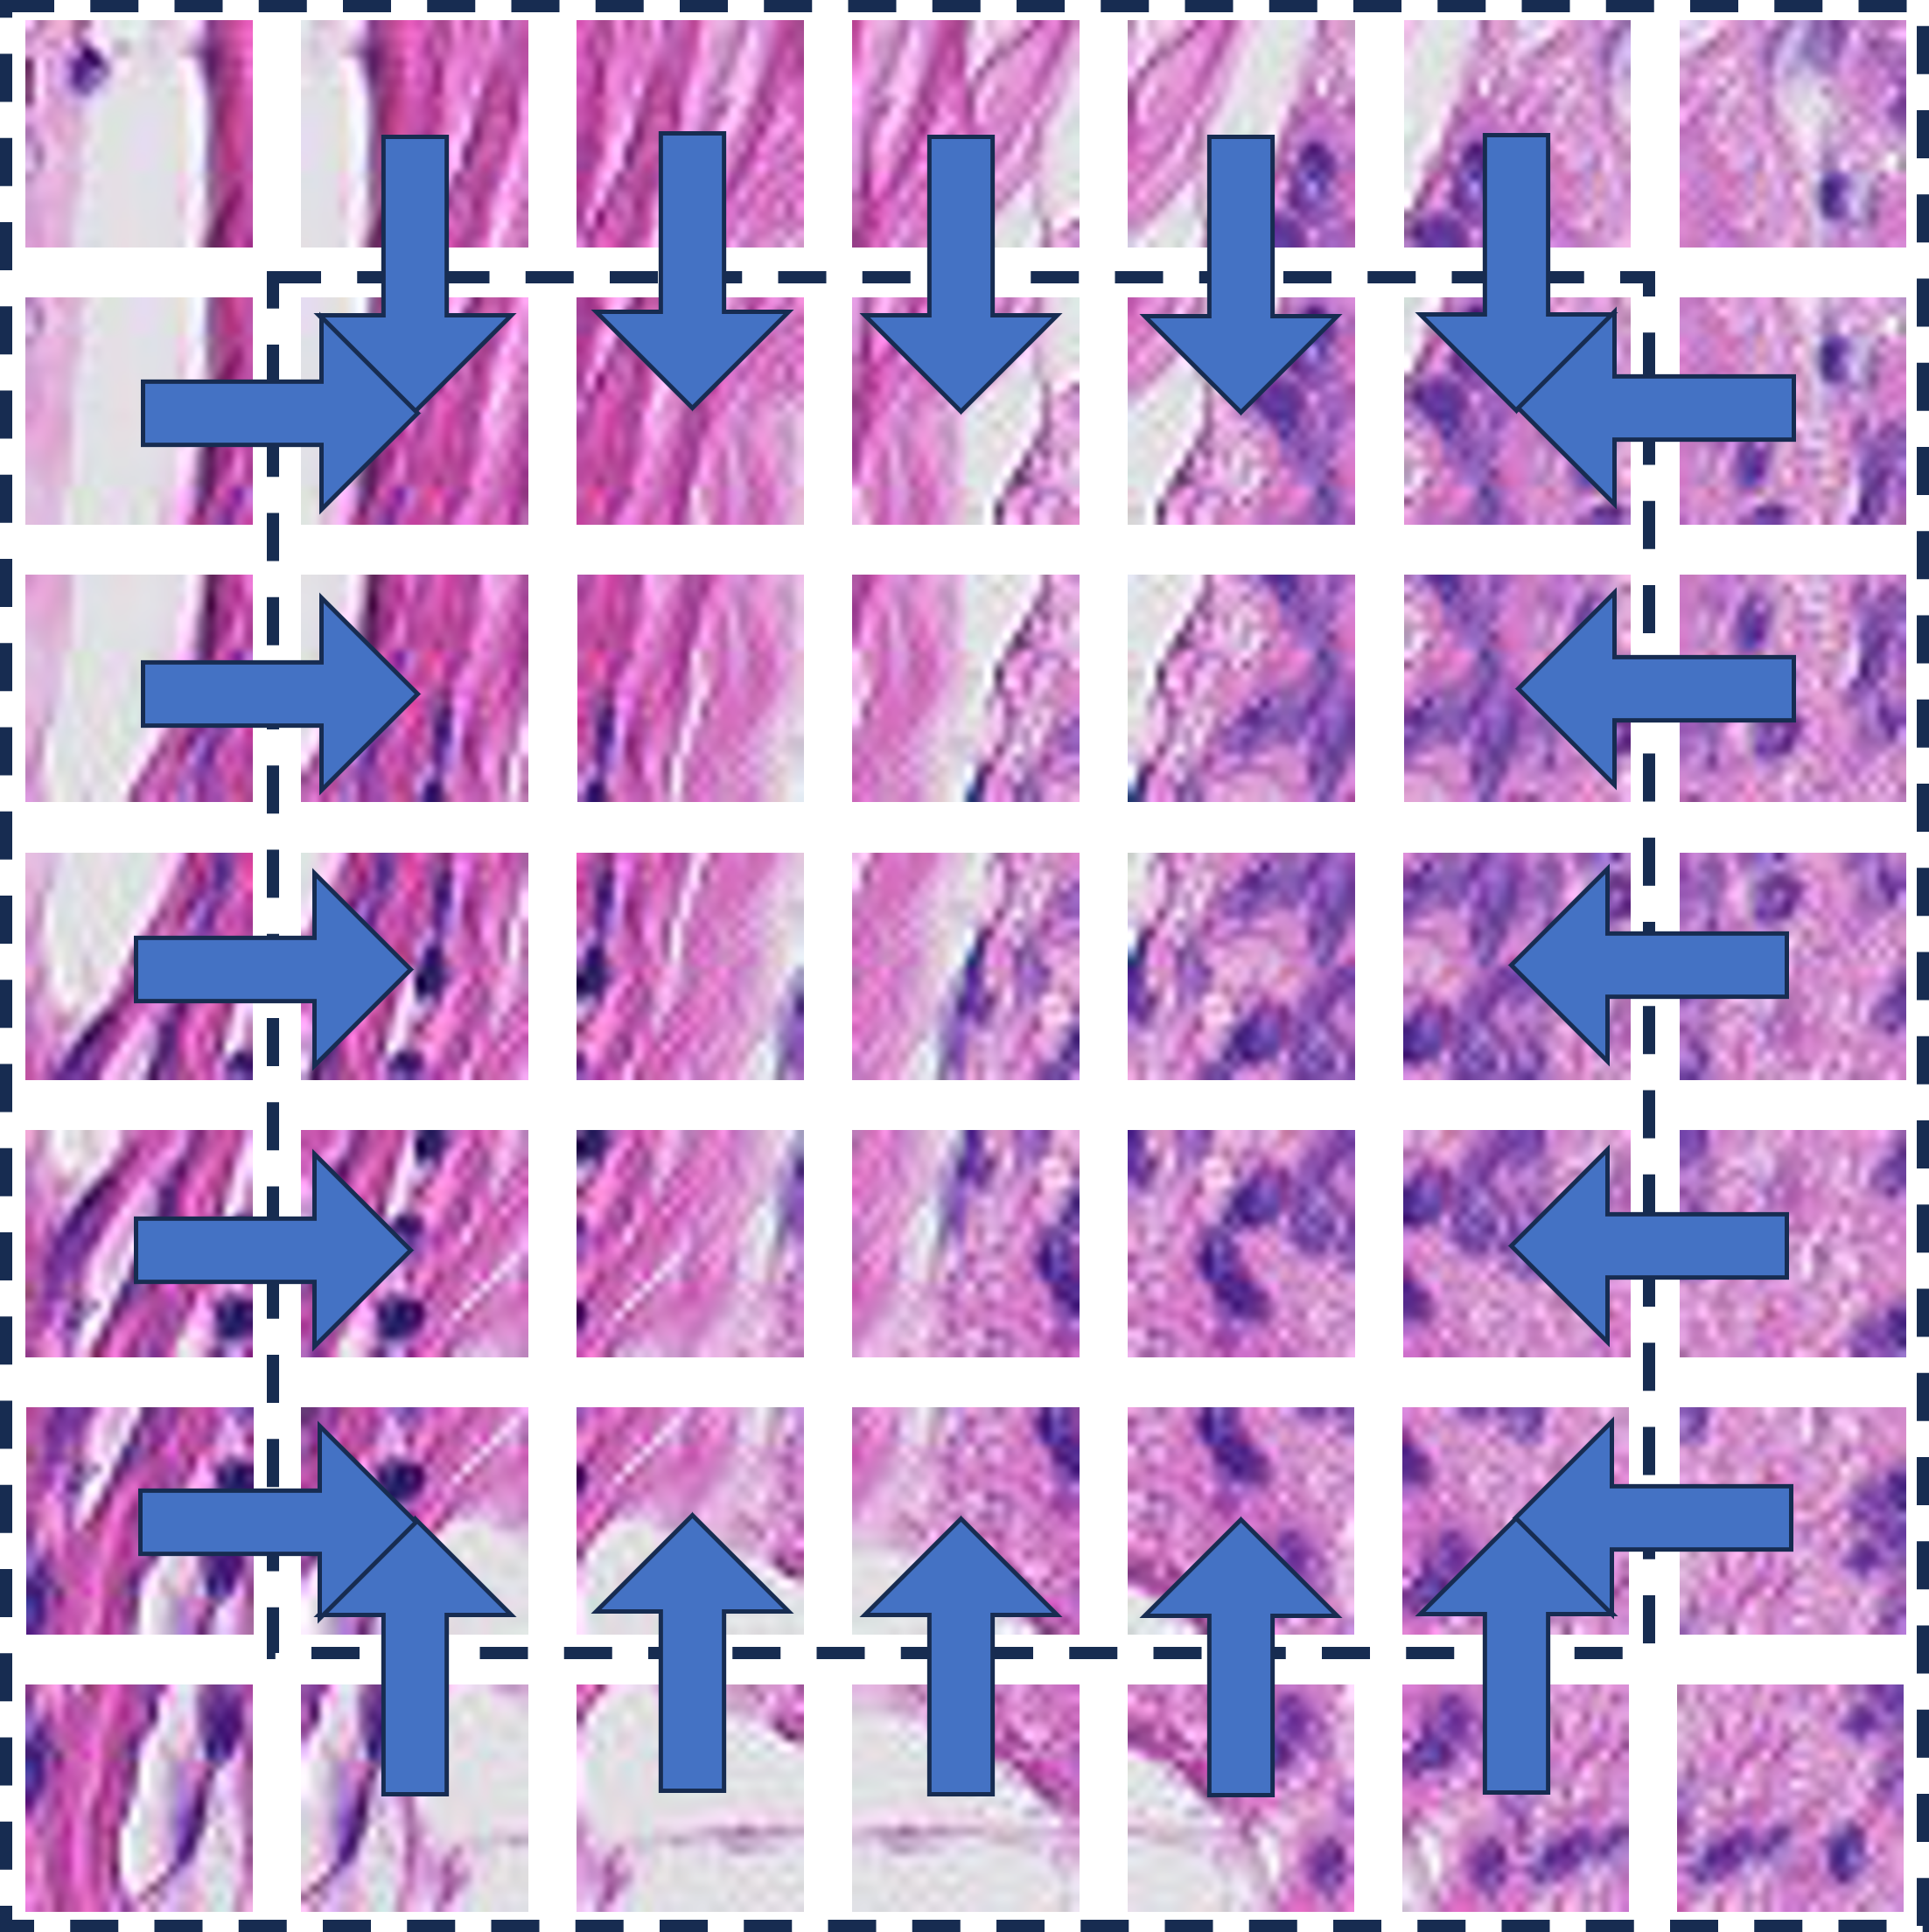
\includegraphics[width=\textwidth]{images/histo_grid.png}}
		\centerline{(d)}\medskip
	\end{minipage}
	\caption{(a) An example image from the ImageNet dataset~\citep{deng2009imagenet}. (b) Extracted overlapping patches with those used to produce context and autoregressor direction highlighted. (c) An example image from the Patch Camelyon dataset~\citep{veeling2018rotation}. (d) Extracted overlapping patches with those used to produce context and autoregressor direction highlighted.}
	\label{fig:example_cpc_patches}
\end{figure}

One approach to reducing the need for large, annotated datasets is through the use of unsupervised representation learning and transfer learning. This is accomplished by using the weights of a deep encoder, trained on a large pool of unannotated data, to initialise another model~\citep{weiss2016survey}. Contrastive predictive coding (CPC) is a state-of-the-art method for unsupervised representation learning~\citep{oord2018representation}. It involves training an autoregressive model to predict future data representations in a sequence, using a loss function with noise-contrastive estimation and importance sampling components, to preserve the density ratio between each sample and its representation. Although originally developed for sequential data, CPC has been adapted for images by splitting each image into overlapping patches and using an encoder to produce a matrix of feature representations. A mask is then applied to the matrix so that an autoregressive model can only see a subset of the feature representations in order to predict the representations of the masked patches from the context available to it. This framework has been applied successfully to object detection and Imagenet classification tasks with modifications to model capacity, layer normalisation, prediction directions, and patch-based augmentations~\citep{henaff2019data}. However, in previous implementations, the autoregressive model’s predictions were made in multiple directions individually, which can be inefficient when dealing with images, such as in digital pathology, where the orientation of the image is arbitrary and does not carry useful information. Figure~\ref{fig:example_cpc_patches}(b) illustrates an example of this framework applied to an image.

\begin{figure}[b]
	\centering
	\includegraphics[width=\textwidth]{images/active_unsupervised_learning.png}
	\caption{Proposed active learning framework with learnt representations from unsupervised representation learning on unannotated data.}
	\label{fig:active_unsupervised_learning_framework}
\end{figure}

The current study builds upon the idea that unsupervised representation learning can be utilised to learn deep representations, which can then be used in conjunction with transfer learning to train a discriminative classifier with limited annotated data (as depicted in Figure~\ref{fig:active_unsupervised_learning_framework}). By implementing this approach, the need for complex deep learning-specific active learning query strategies is mitigated and instead allows for a focus on uncertainty-based querying. In order to realise this approach, a state-of-the-art unsupervised representation learning algorithm for digital pathology images was required. To this end, a multi-directional CPC extension was proposed, which includes an alternative mask for building latent context and a new extension to the autoregressive model PixelCNN~\citep{oord2016pixel} for multi-directional predictions (as depicted in Figure~\ref{fig:example_cpc_patches}(d)). The effectiveness of this modification was demonstrated using the PatchCamelyon dataset~\citep{veeling2018rotation}, derived from the Camelyon16 dataset~\citep{litjens20181399}, where it was shown that classification can be performed with less annotated data when utilising representations learned in this way. 

This work was presented at the IEEE International Symposium on Biomedical Imaging 2021 and published as part of its proceedings \citep{carse2021unsupervised}.



\section{Unsupervised Representation Learning for Computer Vision}
\label{subsec:unsupervised_representation}
This is a brief review of deep unsupervised representation methods for computer vision applications covering generative/reconstructive and self-supervised methods. In the field of deep learning, methods have shown exceptional performance in tasks involving abundant annotated data. However, their performance is known to suffer in scenarios where the supervision is limited. One solution to this issue is to utilise unsupervised learning techniques to learn highly structured data representations, which can lead to more data-efficient models~\citep{lake2015human}.

Deep learning models typically consist of layers that are used for specific tasks, such as classification or regression, and others that are used to encode the data into feature representations, known as encoders. Unsupervised representation learning in deep learning focuses on learning the parameters of the encoder. Once trained, the encoder can be used for transfer learning and applied to tasks such as classification, object detection, or segmentation~\citep{weiss2016survey}.

In the context of computer vision, there are two main approaches to deep representation learning: generative methods and self-supervised learning~\citep{bengio2013representation}. Generative methods aim to learn representative feature encodings by attempting to reconstruct images. On the other hand, self-supervised learning involves training models in a supervised manner using auto-generated annotations for classification or regression tasks.

\subsection{Generative and Reconstructive Methods}
\label{subsec:generative_methods}
Unsupervised representations can be learned through reconstructive methods by encoding input data into a lower-dimensional latent space and subsequently reconstructing the original data from the latent representation. The optimisation of encoder and decoder parameters is achieved through the use of a reconstruction error as a learning signal. In contrast, generative models are capable of generating new data samples that resemble the training data. Specifically, within the realm of medical image analysis, generative models have been employed for image-to-image translation tasks such as converting images from one modality to another~\citep{kaji2019overview}. The surge in popularity of generative models in medical image analysis can be attributed to their ability to learn useful representations from vast quantities of unannotated data, which can then be leveraged to enhance performance on tasks such as segmentation and classification~\citep{yi2019generative}.

\subsubsection{Autoencoders}
\label{subsubsec:autoencoders}
Autoencoders are a class of reconstructive model that employ an encoder to reduce the dimensionality of the input data and a decoder to reconstruct the original data from the reduced representation~\citep{kramer1991nonlinear}. Transfer learning can be achieved by utilising the parameters learned by the encoder and training a new classifier with the encoded representations. One of the most widely used types of autoencoders is the undercomplete autoencoder, which is trained to minimise the reconstruction error by learning a compressed feature representation~\citep{goodfellow2016deep}. Other variations of autoencoders include sparse autoencoders, which are designed to learn sparse representations that have been shown to improve performance when used for transfer learning~\citep{makhzani2013k}. Denoising autoencoders, on the other hand, are trained by corrupting the input data with noise and the goal of the network is to reconstruct the original data without the added noise. This denoising training process forces the encoder and decoder to implicitly learn the underlying structure of the data, which can be beneficial for transfer learning~\citep{bengio2013generalized}.

The final category of autoencoder is the regularised autoencoder, which modifies the traditional autoencoder architecture in order to enhance the model's ability to learn more informative representations and capture relevant information. One of the most widely employed forms of regularised autoencoder is the variational autoencoder, as proposed by \cite{kingma2013auto}. This variant of autoencoder ensures that the latent space possesses desirable properties that enable a generative process by encoding an input image as a distribution over the latent space, as opposed to encoding it into a single point in the latent space. A variational autoencoder is trained by sampling from the encoded latent distribution and decoding it into an output image. The loss function for this model is based on the reconstruction error of the output image and the Kulback-Leibler divergence~\citep{kullback1951information} as the regularisation term.

Most recent work with autoencoders in medical image analysis has been using variational autoencoders as they have shown a high level or performance and have been used for multiple tasks~\citep{wei2020recent}. \cite{akrami2020brain} used a combination of variational autoencoders and transfer learning to build unsupervised lesion detection models for MRI brain scans images and showed their robustness when working with training and testing datasets with different parameters~\citep{thiagarajan2020improving}. 

\subsubsection{Generative Adversarial Networks}
\label{subsubsec:generative_adversarial_networks}
Generative adversarial networks~\citep{goodfellow2014generative} are a class of deep learning models that are designed to generate new samples of data that resemble existing samples from a given dataset. They consist of two main components: a generator network, which produces new samples, and a discriminator network, which attempts to distinguish the generated samples from the real samples. The two networks are trained in an adversarial manner, with the generator attempting to produce samples that the discriminator cannot distinguish from real samples, and the discriminator attempting to correctly identify the generated samples. However, generative adversarial networks are known to be difficult to train, one common problem when training generative adversarial networks is mode collapse, where the generator produces a limited set of outputs that fail to capture the full diversity of the real data distribution. Several techniques, such as Wasserstein generative adversarial networks~\citep{arjovsky2017wasserstein} and gradient penalty~\citep{gulrajani2017improved} have been proposed to stabilise the training process.

In the context of representation learning, generative adversarial networks can be used to learn a compact, low-dimensional representation of the data that captures the underlying structure of the dataset. This can be achieved by training the generator to produce samples that are similar to the real samples, but in a lower-dimensional space. The generator can then be used as a feature extractor, mapping the real samples to their corresponding low-dimensional representations. Additionally, the discriminator can be used as a classifier, allowing the learned representations to be used for downstream tasks such as classification~\citep{srivastav2021improved} or clustering~\citep{mukherjee2019clustergan}.

A variant of generative adversarial networks is BigBiGAN~\citep{donahue2019large}, which is designed to generate high-quality images from a compact, low-dimensional representation of the data. It is based on the idea of BiGAN~\citep{donahue2016adversarial} and the primary difference between BigBiGAN and the original BiGAN is the scale of the model. BigBiGAN is trained on a large dataset such as ImageNet, which contains millions of images, whereas BiGAN is trained on smaller datasets. The increased size of the dataset allows BigBiGAN to learn a more powerful and expressive representation of the data. BigBiGAN consists of three main components: an encoder network, a generator network, and a discriminator network. The encoder network maps the input data to a low-dimensional representation, which is then used as input to the generator network to produce a reconstructed sample.

\subsection{Self-supervised Methods}
\label{subsec:self_supervised_methods}
Self-supervised learning for representation learning is a subset of machine learning that aims to learn meaningful representations of data without the need for explicit annotations. A prevalent method for self-supervised representation learning in medical imaging is to employ a pretext task, a task that is simple to solve through the utilisation of the features learned by the model, but also serves as a means to learn relevant features for the ultimate task of interest. The utilisation of self-supervised pre-training techniques is rapidly gaining popularity in medical image analysis, as it enables the learning of useful features from large amounts of unannotated data, which can then be applied to enhance performance in tasks such as segmentation and classification~\citep{shurrab2022self}.

\subsubsection{RotNet}
\label{subsubsec:RotNet}
RotNet, as proposed by \cite{gidaris2018unsupervised}, is a novel unsupervised representation learning technique that utilises rotation as a self-supervised task for learning useful representations of images. The fundamental concept behind RotNet is that by training a neural network to predict the rotation of an image, it can learn useful features can be utilised in other tasks such as image classification. The RotNet model comprises of a convolutional neural network that takes an image as input and predicts the angle of rotation. The output of the last convolutional layer, prior to the fully connected layers, is used as the representation of the image. This technique enables the model to train on a large dataset of unannotated images, which can then be utilised for other tasks such as image classification as demonstrated by \cite{zhou2021preservational}.

\subsubsection{Deep Clustering}
\label{subsubsec:deep_clustering}
DeepCluster, as proposed by \cite{caron2018deep}, is a technique for unsupervised representation learning that combines the utilisation of clustering algorithms as a form of self-supervision to train deep neural networks. The method starts by initialising the weights of a deep neural network randomly and subsequently utilising the network to extract features from a dataset of unannotated images. These features are then employed to cluster the images into different groups using a clustering algorithm, such as k-means. Upon completion of the clustering process, the annotations generated by the clustering algorithm are used as pseudo-annotations for the images. The neural network is then fine-tuned using these pseudo-annotations to enhance the representations of the images. This process is repeated multiple times, with the neural network being fine-tuned using the updated pseudo-annotations generated by the clustering algorithm.

\subsubsection{Non-Parametric Instance-Level Discrimination}
\label{subsubsec:non-parametric_instance-level_discrimination}
Non-parametric instance-level discrimination is a method for unsupervised representation learning that focuses on learning a set of discriminative features that can be used to differentiate between individual instances in a dataset. This approach is non-parametric, meaning that it does not rely on assumptions about the underlying distribution of the data or the form of the learned features. \cite{wu2018unsupervised} proposed a modification to apply this to deep learning. The authors noted that simply extending the softmax output to the size of the dataset is not feasible and instead found a way around this by approximating the softmax distribution using noise-contrastive estimation~\citep{gutmann2010noise} and using a proximal regularisation method~\citep{parikh2014proximal}.

\subsubsection{Local Aggregation}
\label{subsubsec:local_aggregation}
In their work, \cite{zhuang2019local} proposed a method for unsupervised representation learning using local non-parametric aggregation in the latent feature space. The proposed method is based on training an encoder to produce latent features, and encouraging similar data instances to move together and dissimilar instances to separate in the latent feature space. To achieve this, the method employs a clustering technique. Specifically, multiple passes of k-means clustering are performed for each latent encoding to determine its close neighbours and background neighbours. The loss function used to train the model is based on the negative log-likelihood of an encoding being recognised as a close neighbour, given that it is recognised as a background neighbour. The effectiveness of the proposed method is demonstrated through experiments on the Imagenet dataset~\citep{deng2009imagenet}. The results show that the model trained with this method exhibits substantial ability to recognise high-level visual context without the need for any dataset annotations. This highlights the potential of the proposed method for unsupervised representation learning in computer vision tasks.

\subsubsection{Momentum Contrast}
\label{subsubsec:momentum_contrast}
In their work, \cite{he2020momentum} proposed a method for unsupervised representation learning called momentum contrast. The method uses a dynamic dictionary of keys to train an encoder. Specifically, the encoder is trained using a contrastive loss, which compares the representation of a query image to the key representations from the dynamic dictionary, which is made up of a queue of data samples. The authors claim that the use of a large and dynamic dictionary allows for an effective sampling of high-dimensional visual space, which results in competitive performance. This is supported by the experimental results presented in the work, which show that the learned feature representations can be used to pre-train encoders for a variety of tasks such as classification, detection, and segmentation. This highlights the potential of the Momentum Contrast method for unsupervised representation learning in computer vision tasks.

\subsubsection{Pretext-Invariant Representations}
\label{subsubsec:pretext_invariant_representations}
In a recent study, \cite{misra2020self} highlighted a limitation of using pretext tasks for self-supervised representation learning, specifically that it can result in overfitting and poor generalisation to other tasks. To address this issue, the authors proposed a novel approach called pretext-invariant representation learning. This method involves applying a transformation, such as a rotation, to an input image, and then encoding both the original and transformed images using a shared encoder. The final embeddings are generated using separate prediction heads. To further improve the robustness of the learned representations, the authors employed a noise contrastive estimator~\citep{gutmann2010noise} as the loss function, which aims to reduce the similarity between the original and transformed images, while maximising the similarity between the transformed image and randomly sampled negative images. The encoder used in the study was a ResNet~\citep{he2016deep}, and the authors demonstrated the effectiveness of the proposed approach by achieving state-of-the-art results using a jigsaw pretext task~\citep{noroozi2016unsupervised}, where the model arranges shuffled image patches.

\subsubsection{Deep InfoMax}
\label{subsubsec:DIM}
Deep infomax, first proposed in~\citep{hjelm2018learning}, is a self-supervised deep learning approach for learning compact and informative representations of data through the optimisation of mutual information between the data and the learned representations. Mutual information is a measure of the dependence between two random variables and quantifies the amount of information that one variable contains about the other. In the case of deep infomax, the data is considered as one random variable and the learned representation as the other. The mutual information between the data and the learned representation is estimated using a variational lower bound.

An extension of this approach, Augmented Multiscale Deep InfoMax (AMDIM)~\citep{bachman2019learning}, aims to learn hierarchical representations of data by utilising a multiscale architecture. This architecture is composed of multiple sub-networks, each responsible for learning representations at a different scale. The decoder network also comprises of multiple sub-networks, each responsible for reconstructing the data from the representations at a corresponding scale. Like deep infomax, the mutual information between the data and the learned representations is estimated using a variational lower bound. The key difference between deep infomax and AMDIM is that the latter utilises multiple scales to learn hierarchical representations, while the former only uses one scale. The authors of the paper have demonstrated state-of-the-art results using transfer learning to train classifiers.

\subsection{Unsupervised Representation Learning for \\Medical Image Analysis}
\label{subsec:unsupervise_representation_for_medical}
In the field of digital pathology, transfer learning is a widely used technique for various tasks~\citep{srinidhi2020deep}, as it has been shown to accelerate the convergence of deep learning models~\citep{bayramoglu2016transfer}. Studies have also demonstrated the effectiveness of utilising representation learning to initialise a CNN in situations where the learning task may be challenging due to a lack of annotated data~\citep{hou2016automatic}. This approach can also be extended to active learning, where limited annotations make it difficult to learn features effectively~\citep{carse2019active}.

Instead of relying on features trained on general computer vision data, some researchers have explored the use of more general histology features for cell-level tasks~\citep{hu2018unsupervised}. One method for achieving this is by training a unified generative adversarial network with a modified loss function for cell-level representation learning. Another approach is to use multi-scale convolutional sparse coding, which aims to jointly learn features at different scales with enforced scale-specificity~\citep{chang2017unsupervised}.

Many of the methods under consideration depend on utilising an image’s inherent orientation. However, this approach can prove challenging in instances where an image lacks a natural orientation, such as with histopathology patches or dermoscopic skin lesions. Consequently, there is a need to modify existing methodologies to better accommodate these types of medical images.



\section{Multi-Directional Contrastive Predictive Coding}
\label{sec:unsupervised_multi_directional_cpc}
\subsection{Contrastive Predictive Coding}
\label{subsec:unsupervised_cpc}
CPC is an unsupervised method of feature representation that effectively extracts information from sequential data~\citep{oord2018representation}. The fundamental principle of CPC is to learn 'slow representations' that accurately capture the input data distribution over an extended period, rather than focusing on low-level, local representations. This is achieved by encoding a target variable, denoted by $x$, and a context variable, denoted by $c$, into compact distribution vector representations that maximally preserve information, as shown in Equation~(\ref{eq:mutual_infotmation_cpc}). By maximising $I(x;c)$ between the encoded representations, the underlying latent variables between inputs can be extracted.

\begin{equation}
	I(x;c) = \sum_{x, c}p(x, c) log \frac{p(x|c)}{x}
	\label{eq:mutual_infotmation_cpc}
\end{equation}

A CPC model comprises two essential components, namely an encoder and an autoregressive model. Specifically, the encoder function, denoted by $g_{enc}$, is responsible for encoding each element $x_t$ of the input sequence $x$ into latent representations, which are represented as $z_t = g_{enc}(x_t)$. On the other hand, the autoregressive model function, $g_{ar}$, summarises a portion of the latent representation sequence, $z_{\le t}$, into a latent context representation, which is represented as $c_t = g_{ar}(z_{\le t})$. Rather than utilising the autoregressive model to predict future samples, a density ratio is modelled to maintain the mutual information between $x_{t+k}$ and $c_t$, as elucidated in Equation~(\ref{eq:density_ratio}). By utilising density ratios, the model avoids the need to learn from the high-dimensional input distribution.

\begin{equation}
	f_k(x_{t+k},c_t) \propto \frac{p(x_{t+k}|c_t)}{p(x_{t+k})}
	\label{eq:density_ratio}
\end{equation}

The direct evaluation of $p(x)$ or $p(x|c)$ is not feasible, and therefore, it is necessary to approximate these values using sampling techniques such as noise-contrastive estimation (NCE)~\citep{gutmann2010noise} or importance sampling. The joint training of encoder and autoregressive models using NCE with importance sampling can be facilitated by the InfoNCE loss function (Equation~(\ref{eq:infonce}))~\citep{oord2018representation}, which was introduced by a previous study. Specifically, the InfoNCE loss function involves optimising the density ratio that maintains the mutual information between the context vector $c_t$ and future observations, given a set $X = \{x_1,…,x_N\}$ consisting of one positive sample from $p(x_{t+k}|c_t)$ and N negative samples from the proposed distribution $p(x_{t+k})$. The InfoNCE loss is defined as the cross-entropy of classifying the positive sample correctly.

\begin{equation}
	L_N=-\underset{X}{\mathbb{E}}\left[\log\frac{f_k(x_{t+k},c_t)}{\sum_{x_j\in X}f_k(x_j,c_t)}\right]
	\label{eq:infonce}
\end{equation}


\subsection{Contrastive Predictive Coding for Computer Vision}
\label{subsec:unsupervised_cpc_for_vision}
CPC is a method originally proposed for sequential data, and its application to computer vision involves first dividing an input image into overlapping patches. Each patch is then encoded, and an autoregressive model is employed to generate a context vector from the patch representations at the top of the image (as depicted in Figure~\ref{fig:example_cpc_patches}(b), where the top 3 rows of patches were utilised~\citep{oord2018representation}). This approach treats each column of the image as a sequence, with the context vector from the top of the image used to model the density ratio with patch representations below. This technique has been demonstrated to achieve data-efficient results on high-level computer vision datasets, such as Imagenet~\citep{henaff2019data}.

\subsection{Pixel Convolutional Neural Network}
\label{subsec:pixelcnn}
PixelRNNs~\citep{van2016pixel} and PixelCNNs~\citep{oord2016pixel} are both generative neural networks. These models utilise sequential prediction to generate images by predicting pixels in two spatial dimensions. PixelRNNs and PixelCNNs are designed to model the discrete probability of raw pixel values and capture the full set of dependencies within an image. PixelCNNs, in particular, utilise autoregressive connections to model images pixel by pixel, allowing for the decomposition of the joint image distribution as a product of conditionals. This approach enables PixelCNNs to generate high-quality images that closely resemble the training data. Moreover, PixelCNNs offer a significant advantage over PixelRNNs in terms of training efficiency. This is due to the inherent parallelisability of convolutions, which enable the model to be trained much faster on large image datasets. As a result, PixelCNNs have emerged as a popular and effective approach for generative image modelling.

\subsection{Multi-Directional Contrastive Predictive Coding}
\label{subsec:unsupervised_mdcpc}
The approach of treating columns of the representation matrix as individual sequences (as described in Section~\ref{subsec:unsupervised_cpc_for_vision}), can negatively impact performance when working with images where image orientation is irrelevant, such as histology patches or dermoscopic skin lesion images. While the orientation of certain histology whole slide images can be biologically meaningful, the orientation of image patches, such as those shown in Figure~\ref{fig:fig:example_cpc_patches}(c) (sentinel lymph node), is not important. In such cases, the autoregressive model can struggle to predict patch representation from the provided context as the vertical image axis is arbitrary, unlike Imagenet where it correlates with the direction of gravity acting upon the image content.

\begin{figure}
	\centering
	\includegraphics[width=0.9\textwidth]{mcb.png}
	\caption{Architecture of a Multi-Directional Masked Block}
	\label{fig:multi-directional_masked_block}
\end{figure}

To address this limitation, this work proposes two modifications inspired by image in-filling: an alternative latent mask for producing a context vector, and a modified PixelCNN~\citep{oord2016pixel} for multi-directional context building. The proposed multi-directional CPC utilises these two modifications to more effectively learn representations from images where image rotation is uninformative.

The modified version of the PixelCNN is used as the autoregressive model in a multi-directional CPC model. This modification replaces each masked convolutional block of the PixelCNN architecture with a multi-directional masked blocks (Figure~\ref{fig:multi-directional_masked_block}). Each multi-directional masked block takes a single input image and by rotating 0\textdegree, 90\textdegree, 180\textdegree and 270\textdegree, produces four versions of the original image. A masked block, as described in \cite{oord2016pixel}, is then applied to each of them. The four outputs from the masked blocks are then concatenated and put through a final 1x1 convolutional layer for dimensionality reduction.

This multi-directional autoregressive model is used to learn a latent context from multiple directions at the same time. To take advantage of this, an alternative latent mask inspired by in-filling is introduced. With this mask (illustrated in Figure~\ref{fig:example_cpc_patches}(d), the autoregressive model only has access to the patch representations around the perimeter of the patch representations. This means that images, where rotation is unimportant, can be better represented than with features learned using a single-directional CPC.



\section{Unsupervised Representation Learning Experiments}
\label{sec:unsupervised_experiments}
This section presents a description of the datasets, training parameters, experimental setup, and results from experiments with the proposed multi-directional contrastive predictive coding approach on digital pathology whole-slide patches. The methodology, experimental results and detailed information on the datasets used in this study are provided in a transparent and reproducible manner. The codes and full results used in this section can be accessed on the project's GitHub repository\footnote{GitHub Repository: \url{github.com/UoD-CVIP/Multi_Directional_CPC_Histology}} for further validation, replication and testing by the research community.

\subsection{Dataset}
\label{subsec:unsupervised_dataset}
The publicly available dataset Patch Cameleyon~\citep{veeling2018rotation} was chosen for its suitability to evaluate the proposed method. This dataset was selected due to its large number of non-overlapping whole-slide image patches that possess no inherent directionality, making it a suitable benchmark for evaluating rotation-invariant representations. It was previously used to evaluate Rotation Equivariant CNNs~\citep{velling2018rotation}. The patches were extracted from 400 whole-slide image scans of sentinel lymph node sections from the Camelyon16 dataset~\citep{litjens20181399}. These whole-slide images were collected from two centres in the Netherlands (Radboud University Medical Center\footnote{Radboud University Medical Center: \url{www.radboudumc.nl}} and University Medical Center Utrecht\footnote{University Medical Center Utrecht: \url{www.umcutrecht.nl}}) and digitised using an objective of 40x magnification, resulting in a pixel resolution of 0.243 microns. Each patch has been annotated with a binary annotation indicating the presence or absence of metastatic tissue, by determining if the centred 32x32 pixels of the patch contains at least one pixel of tumour. The dataset is balanced between the two binary classification. The dataset contains a total of 327,680 patches which were split into training and testing sets, with a ratio of 90:10. To improve generalisation, data augmentation was applied during training, by randomly rotating, flipping vertically, and flipping horizontally each patch during sampling.

\begin{figure}
	\centering
	\begin{subfigure}{\textwidth}
		\centering
		\includegraphics[width=0.3\linewidth]{images/pcam_0_0.png}
		\includegraphics[width=0.3\linewidth]{images/pcam_79_0.png}
		\includegraphics[width=0.3\linewidth]{images/pcam_13_0.png}
		\caption{Negative Examples}
	\end{subfigure}
	\begin{subfigure}{\textwidth}
	\centering
	\includegraphics[width=0.3\linewidth]{images/pcam_1_1.png}
	\includegraphics[width=0.3\linewidth]{images/pcam_78_1.png}
	\includegraphics[width=0.3\linewidth]{images/pcam_22_1.png}
	\caption{Positive Examples}
\end{subfigure}
	\caption{Example images from the Patch Cameleyon dataset~\citep{veeling2018rotation,litjens20181399}.}
	\label{fig:pcam_examples}
\end{figure}

\subsection{Experiment Setup}
\label{subsec:unsupervised_experiment}
In order to evaluate the proposed multi-directional contrastive predictive coding approach, an ablation study was conducted using different combinations of the single or multi-directional autoregressive models, and top-down or in-filling style latent masks. To evaluate the learned representations from the CPC models, the trained encoders were used to initialise the encoder weights of 9 CNN classifiers. These CNN classifiers were then trained on a smaller, annotated subset of the training data, which was varied in size from 10 to 100,000 patches in logarithmic scale. This was repeated 3 times, each time with a different subsample of the training data to validate the robustness of the results. The test set was held static across all experiments.

\subsection{Training Parameters}
\label{subsec:unsupervised_training}
The CPC models were trained using a method that involved splitting each input image into overlapping 24x24 patches that overlapped their neighbours by 12 pixels. A ResNeXt architecture with 101 layers was utilised as the encoder, followed by an additional convolutional layer to produce a 128-dimensional feature vector for each 24x24 patch in the image. The autoregressive model of the CPC was composed of 6 masked convolutional blocks to produce the context vector and predict the masked feature vectors. Additionally, 16 randomly selected images were used as negative samples for the CPC InfoNCE loss function.

The Adam optimisation algorithm was utilised to train the CPC and CNN models, with an initial learning rate of 1e-4. The Adam optimiser~\citep{kingma2014adam} is based on adaptive estimation of first and second-order moments in the parameter gradients to adjust the learning rate during training. The CPC model was trained for 10 epochs with a batch size of 64 and the CNN models were trained for 50 epochs with a batch size of 258. 20\% of the available training data was used as the validation set to prevent overfitting, and early stopping was implemented by saving the model when the loss was lowest on the validation set. 

The CPC models took an average of 33 hours to train using a single Nvidia GeForce RTX 2080 Ti using 16-bit precision. The training loss over the epochs (Figure~\ref{fig:cpc_training}) suggests that the use of a multi-directional autoregressive model was more efficient at reducing the InfoNCE loss than a single-directional top-down autoregressive model. The in-filling style latent mask in combination with the multi-directional autoregressive model stabilised the CPC training process.

\begin{figure}[h]
	\centering
	\includegraphics[width=\textwidth]{images/cpc_training.png}
	\caption{Training loss each epoch with the CPC Models.}
	\label{fig:cpc_training}
\end{figure}

\begin{table}[h]
	\centering
	\caption{Mean test accuracies of the CNN classifiers with different pre-training (standard deviation in parentheses).}
	\label{tab:cpc_cnn_results}
	\resizebox{\textwidth}{!}{%
		\begin{tabular}{r|rrrrr}
			\multicolumn{1}{c|}{\begin{tabular}[c]{@{}c@{}}Training\\ Examples\end{tabular}} &
			\multicolumn{1}{c}{\begin{tabular}[c]{@{}c@{}}No \\ Pretraining\end{tabular}} &
			\multicolumn{1}{c}{\begin{tabular}[c]{@{}c@{}}Single\\Directional\\Normal Mask\end{tabular}} &
			\multicolumn{1}{c}{\begin{tabular}[c]{@{}c@{}}Single\\Directional\\Infilling Mask\end{tabular}} &
			\multicolumn{1}{c}{\begin{tabular}[c]{@{}c@{}}Multi\\Directional\\Normal Mask\end{tabular}} &
			\multicolumn{1}{c}{\begin{tabular}[c]{@{}c@{}}Multi\\Directional\\Infilling Mask\end{tabular}} \\ \hline
			10     & 0.500 (0.000) & 0.561 (0.043)          & 0.561 (0.094)          & 0.546 (0.065)          & \textbf{0.582 (0.096)} \\
			32     & 0.563 (0.109) & 0.560 (0.045)          & \textbf{0.604 (0.043)} & 0.538 (0.082)          & 0.577 (0.086)          \\
			100    & 0.641 (0.125) & 0.590 (0.018)          & 0.636 (0.082)          & 0.595 (0.078)          & \textbf{0.655 (0.081)} \\
			316    & 0.694 (0.067) & 0.593 (0.109)          & \textbf{0.741 (0.014)} & 0.715 (0.039)          & 0.708 (0.062)          \\
			1000   & 0.727 (0.013) & 0.758 (0.014)          & 0.740 (0.016)          & 0.760 (0.016)          & \textbf{0.773 (0.006)} \\
			3162   & 0.750 (0.002) & 0.777 (0.028)          & 0.775 (0.012)          & 0.784 (0.006)          & \textbf{0.786 (0.014)} \\
			10000  & 0.786 (0.006) & 0.787 (0.008)          & 0.776 (0.012)          & \textbf{0.792 (0.033)} & 0.781 (0.019)          \\
			31624  & 0.779 (0.012) & 0.774 (0.004)          & 0.770 (0.009)          & \textbf{0.786 (0.005)} & 0.784 (0.009)          \\
			100000 & 0.775 (0.007) & 0.774 (0.011)          & \textbf{0.786 (0.003)} & 0.785 (0.006)          & 0.784 (0.010)
		\end{tabular}%
	}
\end{table}

\subsection{Results}
\label{subsec:unsupervised_results}
The results obtained from the held-out testing set, consisting of 32,768 images, for the CNN classifiers initialised with various CPC encoders' weights and biases are presented in Figure~\ref{fig:cpc_cnn_results} and Table~\ref{tab:cpc_cnn_results}. In addition, a baseline approach was employed, which utilised CNN models with no pretraining. The outcomes demonstrate that the CNNs trained with a small amount of annotated data exhibit higher accuracies when initialised with a multi-directional autoregressive model. However, the standard CPC encounters challenges in learning a representation that is suitable for initialising a CNN classifier, leading to lower accuracies in some instances compared to those initialised using random weights. The results suggest that the transfer learning approach utilising CPC pretraining is most effective when the number of annotated images is limited, as the benefit of using the CPC pretraining diminishes as the number of images increases. Moreover, Table~\ref{tab:cpc_cnn_results} depicts the ablation results obtained by employing two components: infilling style mask and a multi-directional autoregressive model. The findings indicate that using an infilling style mask is the most critical component as both models that include infilling style masks achieve the best results. However, the CPC model utilising a multi-directional autoregressive model and a normal mask performs optimally when larger subsets of the dataset are utilised.

\begin{figure}[h]
	\centering
	\includegraphics[width=\textwidth]{images/cpc_cnn_results.png}
	\caption{Mean class testing accuracies of the CNN classifiers trained using varying amounts of training examples, with standard errors.}
	\label{fig:cpc_cnn_results}
\end{figure}



\section{Conclusion}
\label{sec:conclusion}
The experimental results presented in Section~\ref{subsec:unsupervised_results} demonstrate that the original implementation of CPC~\citep{oord2018representation} does not perform well on patch-based digital pathology tasks. The proposed multi-directional modifications to the CPC, however, yielded better results and improved classification accuracies when annotated data were limited. These experiments illustrate that algorithms based on an assumption of image directionality, as is common in standard computer vision datasets such as CIFAR~\citep{krizhevsky2009learning} and ImageNet~\citep{deng2009imagenet}, may not perform well on images without such directionality. The results of this study suggest that the proposed multi-directional CPC method can be applied to other visual tasks where image orientation is unimportant, as is the case in multiple biomedical imaging settings.
	
	
	\chapter{Predictive Probability Calibration}
	\label{ch:classification_claibration}
	\section{Introduction}
\label{sec:calibration_introduction}
This work was presented at the Uncertainty for Safe Utilization of Machine Learning in Medical Imaging (UNSURE) workshop hosted at Medical Image Computing and Computing Assisted Intervention 2022 (MICCAI) and published as part of the workshop proceedings \citep{carse2022calibration}.

Deep learning classifiers have been widely adopted for medical image analysis tasks such as diagnostic decision support, in certain restricted settings even outperforming medical specialists, e.g., binary classification of dermoscopic melanoma and nevi images~\citep{maron2019systematic}. Such promising results notwithstanding, further improvements are desirable to enable robust translation to the clinic. A known problem with deep neural network classifiers is that they can be poorly calibrated, typically resulting in over-confident predictions. Mis-calibration represents deviation between confidence and correctness. A model that is not well-calibrated cannot correctly identify the amount of uncertainty in its prediction. Well-calibrated probabilistic outputs are needed to support cost-sensitive and selective clinical decision-making~\citep{carse2021robust}, providing information helpful for avoiding adverse outcomes. Calibrated predictions are relevant for active learning~\citep{carse2019active}, reinforcement learning~\citep{dai2020federated} and out-of-distribution detection~\citep{ulmer2020trust}.

Several methods have been reported to improve the calibration of deep classifiers in medical image classification. However, their performance can be inconsistent and evidence for which to adopt for any given task and dataset is somewhat lacking. We present an empirical study that adds to this evidence base, focusing on classification datasets from dermatology and histopathology. 

Temperature scaling~\citep{guo2017calibration} is the most popular method for calibrating modern neural networks due to its post-hoc nature, simple implementation, and effectiveness. It works by scaling output logits using a temperature parameter that is optimized on a validation set. The original implementation called for optimizing temperature using negative log-likelihood. Other researchers have mentioned using calibration metrics to optimize temperature and have stated in passing that this led to improved calibration~\citep{mukhoti2020calibrating,frenkel2021network}. In this paper, we investigate this claim empirically using a density-based estimator for expected calibration error, and an estimator for maximum calibration error. Section~\ref{sec:calibration_measures} briefly discusses these calibration measures. We explore the effect of the use of different metrics for temperature optimization. We do this not only for neural networks trained by minimizing cross-entropy with one-hot encoded target labels but also for networks trained using focal loss and label smoothing. We also compare these with two Bayesian neural networks, based on Bayes-by-Backprop and a Laplace approximation method. These methods are described in Section~\ref{sec:calibration_review}. Details of our experiment design are provided in Section~\ref{sec:calibration_experiments}. Results on the ISIC 2019 multi-class dermatology dataset and the large Patch-Camelyon binary histopathology dataset are given in Section~\ref{subsec:calibration_results}, providing evidence on the relative performance of the methods in terms of calibration and accuracy on two contrasting tasks.



\section{Measures of Calibration}
\label{sec:calibration_measures}
Various metrics can be used to evaluate model calibration. The expected calibration error (ECE)~\citep{guo2017calibration} is a measure of the difference in expectation between the predictive confidence and classification accuracy. A commonly used estimator for ECE splits the probability interval into equally spaced bins. It then takes a weighted average of the absolute differences between the accuracy of the predictions in a bin and the mean of the probabilities in that bin. If we instead compute the maximum of this error over the bins, we obtain the maximum calibration error (MCE). This measure can be useful in high-risk situations where the worst-case calibration is relevant. 

While histogram-based estimation of ECE has proven useful for evaluating calibration~\citep{muller2019does}, others have criticized the use of equally spaced histogram binning because of inherent bias and statistical inefficiency. To address these criticisms, methods for adapting the number and sizes of bins have been proposed ~\citep{roelofs2022mitigating}. An alternative is to replace the use of histograms with continuous density estimators~\citep{zhang2020mix}. KDE-ECE uses kernel density estimation~\citep{parzen1962estimation} to estimate the densities of accuracy and confidence, achieving better data-efficiency. In this paper, we use KDE-ECE with a triweight kernel.

The negative log-likelihood is often utilized as a loss function for optimizing deep neural network classifiers, measuring a probabilistic model's quality by assessing its ability to recover the ground-truth conditional distribution. Negative log-likelihood can also be used as an indicator of a model's calibration.



\section{Calibration Methods and Literature Review}
\label{sec:calibration_review}
Methods that try to improve calibration can be roughly categorized into three broad approaches: regularization methods, post-processing methods, and methods designed to cope inherently with model uncertainty, such as Bayesian neural networks~\citep{gawlikowski2021survey}.


\subsection{Model Regularisation For Calibration}
Model regularization is performed by modifying the objective function used to optimize a model or by altering the dataset to encourage a model to be more robust and better calibrated. Dataset regularization methods have become commonplace with strategies such as data augmentation~\citep{hendrycks2019augmix} or adding out-of-distribution data to the training data~\citep{hendrycks2018deep}. We make use of data augmentation. In our experiments, we compare label smoothing and focal loss, two methods that can improve calibration.

Neural network classifiers are usually trained using a one-hot label encoding. This involves minimizing the expected cross-entropy between target outputs $t_k$ and the network outputs $y_k$, where $t_k=1$ for the true class and $t_k=0$ for the other classes. Label smoothing instead trains a network by minimizing the expected cross-entropy using modified targets $\hat{t} = (1 - \alpha) t + \frac{\alpha}{C}$ where $C$ is the number of classes and $\alpha$ is a free parameter~\citep{szegedy2016rethinking}. Label smoothing thus modifies the target class distribution and $\alpha$ controls the level of smoothing. At the extremes, $\alpha = 1$ results in a uniform distribution and $\alpha = 0$ recovers one-hot encoding. Label smoothing has been used in medical image analysis to improve calibration and robustness to out-of-distribution data~\citep{islam2021spatially}. Its popularity is partly due to ease of implementation and negligible computational overhead. 

Focal loss~\citep{lin2017focal} is a loss function that was originally introduced to improve the performance of object detection by encouraging a model to focus on samples with lower confidence. It has been shown to improve model calibration~\citep{mukhoti2020calibrating}. It weights predictions based on their confidence to encourage the model to learn more from examples closer to the decision boundary. This can reduce overconfidence, improve calibration, and lead to better results with unbalanced datasets. Focal loss can be written as $FL(y) = -\alpha(1-y)^\gamma\log(y)$. It adds the factor $(1-y)^\gamma$ to cross-entropy to weight the predictions. There are two hyper parameters: $\gamma>0$ determines the weighting of less confident examples, and $\alpha \in [0, 1]$ is used to improve the numerical stability.


\subsection{Post-Hoc Calibration}
Temperature scaling~\citep{guo2017calibration} is the most popular post-hoc calibration method for modern neural networks and has been used successfully in medical image analysis~\citep{liang2020improved}. It is a single-parameter version of Platt logistic scaling~\citep{platt1999probabilistic}. It applies a learned temperature parameter, $T > 0$, to rescale the output logits $z$ of a neural network before a softmax activation function is applied to output probabilistic predictions $\hat{y}$~(\ref{eq:temperature_scaling}). $T=1$ recovers the standard softmax activation. Since $T$ is used to scale all the logits, the output $\hat{y}$ has a monotonic relationship with the unscaled output. For this reason, classification accuracy is unaffected by temperature scaling.

\begin{equation}
	\hat{y} = \frac{e^{z/T}}{\sum^{J}_{j=1}e^{z_j/T}}
	\label{eq:temperature_scaling}
\end{equation}

The original implementation of temperature scaling optimizes $T$ by minimizing the negative log-likelihood of the predictions (expected cross-entropy) on a validation set. We have chosen to experiment with the use of alternative metrics for optimizing $T$. It seems reasonable to expect that optimizing $T$ for a calibration measure on a validation set will lead to better test calibration using that measure. Further details will be given in Section~\ref{sec:calibration_experiments}.


\subsection{Bayesian Approximation}
Bayesian neural networks infer distributions over their weight parameters rather than the usual point estimates. Monte Carlo sampling can then be used to approximate predictive distributions and obtain estimates of predictive means and uncertainty measures such as variance. Bayesian neural nets have been used in medical applications for improved calibration and uncertainty estimation~\citep{kwon2020uncertainty}.

Bayes by Backprop~\citep{blundell2015weight} trains a Bayesian neural network whilst using back-propagation to calculate gradients. It uses variational inference to approximate a posterior distribution over weights $q(w|\theta)$. The parameters for the distribution $\theta$ can be computed by minimizing the KL-Divergence between a variational posterior and the true posterior. As there is no way of knowing the true posterior, it is estimated using Monte Carlo sampling of the evidence lower bound. This is shown in Equation~(\ref{eq:elbo}) where $D$ is the dataset and $N$ is the number of Monte Carlo samples.

\begin{equation}
	\text{ELBO}(D, \theta) \approx \sum^N_{n=1}\log q(w^i|\theta)-\log p(w^i) - \log p(D|w^i)
	\label{eq:elbo}
\end{equation}

To train the Bayesian neural network the ELBO is used as part of a loss function alongside cross-entropy. The ELBO is weighted when combined with cross-entropy with the weighting of $\pi_m = \frac{2^{M-m}}{2^M-1}$ where $M$ is the number of batches and $m$ is the current batch. This weighting means that the first few batches are more influenced by the Bayesian complexity and the later batches learn more from the data. 

Laplace approximation~\citep{mackay1992bayesian} is a cost-effective method for training a Bayesian neural network by approximating the posterior as a Gaussian centered at a local maximum. This local maximum is obtained by training using a gradient-based optimiser in the usual way. Curvature is estimated using approximations to the Hessian matrix~\citep{botev2017practical} at the maximum. Thus, a Laplace approximation is fitted post-hoc onto a trained neural network so that probabilistic predictions can be sampled. Laplace approximation has become increasingly popular for Bayesian inference due to its ability to be added post-hoc and its low computational expense compared to other approximations such as Bayes by Backprop~\citep{daxberger2021laplace}.



\section{Calibration Experiments}
\label{sec:calibration_experiments}
This section details the datasets, training parameters, experimental setup, and results for the experiments with different methods for model calibration for medical image analysis. The code and full results used within this section can be found on the project GitHub repository\footnote{GitHub Repository: \url{github.com/UoD-CVIP/Medical_Calibration}}.

\subsection{Datasets}
Our experiments utilize two datasets, the ISIC 2019 challenge dataset~\citep{codella2018skin,combalia2019bcn20000,tschandl2018ham10000} and the Patch Camelyon (PCam) dataset~\citep{veeling2018rotation}. The ISIC 2019 dataset consists of 25,331 dermoscopic skin lesion images of 8 diagnostic classes: melanoma, melanocytic nevus, basal cell carcinoma, actinic keratosis, benign keratosis, dermatofibroma, vascular lesion, and squamous cell carcinoma. The PCam dataset is comprised of 327,680 96x96 pixel image patches extracted from whole-slide images of H\&E-stained lymph node sections from the Camelyon16 dataset~\citep{bejnordi2017diagnostic}. The datasets were split into training, validation and testing sets with proportions 6:2:2. The ISIC images were pre-processed by center-cropping their width to be equal to their height and then resizing to $256 \times 256$ pixels. Both datasets were augmented by normalizing each of the image channels, randomly flipping both horizontally and vertically, and randomly rotating by multiples of 90\textdegree.


\subsection{Experiment Setup}
We trained seven different types of CNN classifier on both the ISIC 2019 and the PCam datasets. In the case of ISIC 2019, each classifier was trained three times using different random seeds that altered the training, validation and testing data splits as well as the neural network weights initialization. The first classifier type, which we refer to as the baseline model, was trained using a standard cross-entropy function with one-hot label encoding. The next two classifiers used label smoothing (LS) with cross-entropy, with $\alpha$ set to $0.1$ and $0.2$, respectively. A further two classifiers types were trained using focal loss (FL) with $\gamma$ set to $2.0$ and $5.0$, respectively. We applied temperature scaling to each of these model types after training. In each case, we optimized the temperature parameter for various measures of calibration. These were the negative log-likelihood (nll), KDE-ECE (ece), and MCE (mce), as well as additive combinations of these three measures. We denote these using TS followed by an abbreviation for the measure used to optimize temperature, e.g., {\em TS nll+mce}. The temperature parameter was optimized using a Limited-memory BFGS optimizer~\citep{liu1989limited}. For comparison, two types of Bayesian neural networks were also trained. These used Bayes-by-Backprop and Laplace approximation, respectively.


\subsection{Training Parameters}
We used an EfficientNet~\citep{tan2019efficientnet} encoder with a compound coefficient of 7, pre-trained on ImageNet~\citep{deng2009imagenet} followed by a fully connected hidden layer with a width of 512 neurons before the output layer. For Bayesian convolutional neural networks, the final hidden and output fully-connected layers are replaced with Bayesian fully-connected layers that learn distributions for the weights and biases to be sampled from. All training used a cyclical learning rate scheduler with scheduling between $10^{-4}$ and $10^{-1}$. The batch size was 16 for the ISIC 2019 data and 64 for the PCam data. Bayes by backprop used a weighted loss function combining the expected lower bound from 10 forward-propagation passes and cross-entropy of the 10 predictions. The Laplace approximation was optimized post-hoc to a trained convolutional neural network model fitting the approximation on the output layer of the model using a full Hessian structure. Each model was trained for 40 epochs and the model with the best validation loss was used for evaluation.


\subsection{Results}
\label{subsec:calibration_results}

\begin{table}[h!]
	\centering
	\caption{Calibration and accuracy results for ISIC 2019 and PCam datasets. ISIC 2019 results are means and standard deviations over three iterations. Each section reports results from a single model type; TS denotes temperature scaling.}
	\label{tab:calibration_results}
	\resizebox{\textwidth}{!}{%
		\begin{tabular}{l|cccc|m{0.8cm}m{0.8cm}m{0.8cm}m{0.8cm}|}
			& \multicolumn{4}{c|}{ISIC 2019} & \multicolumn{4}{c|}{PCam} \\\cline{2-9} 
			& \multicolumn{1}{c|}{KDE-ECE} & \multicolumn{1}{c|}{MCE} & \multicolumn{1}{c|}{NLL} & ACC & \multicolumn{1}{m{0.9cm}|}{KDE-ECE} & \multicolumn{1}{m{0.9cm}|}{MCE} & \multicolumn{1}{m{0.9cm}|}{NLL} & \multicolumn{1}{m{0.9cm}|}{ACC} \\ \hline
			Baseline CNN & \multicolumn{1}{c|}{$0.046 \pm 0.017$} & \multicolumn{1}{c|}{$0.112 \pm 0.042$} & \multicolumn{1}{c|}{$0.514 \pm 0.015$} & \multicolumn{1}{c|}{$0.836 \pm 0.012$} & \multicolumn{1}{c|}{0.123} & \multicolumn{1}{c|}{0.187} & \multicolumn{1}{c|}{0.543} & \multicolumn{1}{c|}{0.848} \\
			TS nll & \multicolumn{1}{c|}{$0.015 \pm 0.002$} & \multicolumn{1}{c|}{$0.037 \pm 0.014$} & \multicolumn{1}{c|}{$0.471 \pm 0.017$} & \multicolumn{1}{c|}{$0.836 \pm 0.012$} & \multicolumn{1}{c|}{0.123} & \multicolumn{1}{c|}{0.187} & \multicolumn{1}{c|}{0.543} & \multicolumn{1}{c|}{0.848} \\
			TS ece & \multicolumn{1}{c|}{$0.017 \pm 0.007$} & \multicolumn{1}{c|}{$0.038 \pm 0.010$} & \multicolumn{1}{c|}{$0.472 \pm 0.017$} & \multicolumn{1}{c|}{$0.836 \pm 0.012$} & \multicolumn{1}{c|}{0.123} & \multicolumn{1}{c|}{0.204} & \multicolumn{1}{c|}{0.585} & \multicolumn{1}{c|}{0.848} \\
			TS mce & \multicolumn{1}{c|}{$0.016 \pm 0.004$} & \multicolumn{1}{c|}{$0.042 \pm 0.009$} & \multicolumn{1}{c|}{$0.471 \pm 0.018$} & \multicolumn{1}{c|}{$0.836 \pm 0.012$} & \multicolumn{1}{c|}{0.123} & \multicolumn{1}{c|}{0.197} & \multicolumn{1}{c|}{0.567} & \multicolumn{1}{c|}{0.848} \\
			TS nll+ece & \multicolumn{1}{c|}{$0.012 \pm 0.002$} & \multicolumn{1}{c|}{$0.043 \pm 0.012$} & \multicolumn{1}{c|}{$0.471 \pm 0.017$} & \multicolumn{1}{c|}{$0.836 \pm 0.012$} & \multicolumn{1}{c|}{0.122} & \multicolumn{1}{c|}{0.210} & \multicolumn{1}{c|}{0.603} & \multicolumn{1}{c|}{0.848} \\
			TS nll+mce & \multicolumn{1}{c|}{$0.018 \pm 0.002$} & \multicolumn{1}{c|}{$0.038 \pm 0.010$} &  \multicolumn{1}{c|}{$0.472 \pm 0.018$} & \multicolumn{1}{c|}{$0.836 \pm 0.012$} & \multicolumn{1}{c|}{0.123} & \multicolumn{1}{c|}{0.210} & \multicolumn{1}{c|}{0.605} & \multicolumn{1}{c|}{0.848} \\
			TS ece+mce & \multicolumn{1}{c|}{$0.014 \pm 0.021$} & \multicolumn{1}{c|}{$0.041 \pm 0.014$} & \multicolumn{1}{c|}{$0.472 \pm 0.017$} & \multicolumn{1}{c|}{$0.836 \pm 0.012$} & \multicolumn{1}{c|}{0.123} & \multicolumn{1}{c|}{0.193} & \multicolumn{1}{c|}{0.557} & \multicolumn{1}{c|}{0.848} \\
			TS nll+ece+mce & \multicolumn{1}{c|}{$0.015 \pm 0.003$} & \multicolumn{1}{c|}{$0.042 \pm 0.011$} & \multicolumn{1}{c|}{$0.472 \pm 0.017$} & \multicolumn{1}{c|}{$0.836 \pm 0.012$} & \multicolumn{1}{c|}{0.123} & \multicolumn{1}{c|}{0.187} & \multicolumn{1}{c|}{0.543} & \multicolumn{1}{c|}{0.848} \\\hline \hline
			LS $\alpha=0.1$ & \multicolumn{1}{c|}{$0.039 \pm 0.001$} & \multicolumn{1}{c|}{$0.065 \pm 0.001$} & \multicolumn{1}{c|}{$0.495 \pm 0.011$} & \multicolumn{1}{c|}{$0.855 \pm 0.005$} & \multicolumn{1}{c|}{0.116} & \multicolumn{1}{c|}{0.146} & \multicolumn{1}{c|}{0.398} & \multicolumn{1}{c|}{0.848} \\
			TS nll & \multicolumn{1}{c|}{$0.028 \pm 0.003$} & \multicolumn{1}{c|}{$0.087 \pm 0.021$} & \multicolumn{1}{c|}{$0.483 \pm 0.013$} & \multicolumn{1}{c|}{$0.855 \pm 0.005$} & \multicolumn{1}{c|}{0.123} & \multicolumn{1}{c|}{0.244} & \multicolumn{1}{c|}{0.536} & \multicolumn{1}{c|}{0.848} \\
			TS ece & \multicolumn{1}{c|}{$0.029 \pm 0.003$} & \multicolumn{1}{c|}{$0.134 \pm 0.023$} & \multicolumn{1}{c|}{$0.504 \pm 0.013$} & \multicolumn{1}{c|}{$0.855 \pm 0.005$} & \multicolumn{1}{c|}{0.124} & \multicolumn{1}{c|}{0.346} & \multicolumn{1}{c|}{1.112} & \multicolumn{1}{c|}{0.848} \\
			TS mce & \multicolumn{1}{c|}{$0.053 \pm 0.016$} & \multicolumn{1}{c|}{$0.070 \pm 0.016$} & \multicolumn{1}{c|}{$0.505 \pm 0.004$} & \multicolumn{1}{c|}{$0.855 \pm 0.005$} & \multicolumn{1}{c|}{0.121} & \multicolumn{1}{c|}{0.198} & \multicolumn{1}{c|}{0.423} & \multicolumn{1}{c|}{0.848} \\
			TS nll+ece & \multicolumn{1}{c|}{$0.028 \pm 0.003$} & \multicolumn{1}{c|}{$0.086 \pm 0.020$} & \multicolumn{1}{c|}{$0.048 \pm 0.013$} & \multicolumn{1}{c|}{$0.855 \pm 0.005$} & \multicolumn{1}{c|}{0.123} & \multicolumn{1}{c|}{0.237} & \multicolumn{1}{c|}{0.551} & \multicolumn{1}{c|}{0.848} \\
			TS nll+mce & \multicolumn{1}{c|}{$0.033 \pm 0.006$} & \multicolumn{1}{c|}{$0.071 \pm 0.016$} & \multicolumn{1}{c|}{$0.490 \pm 0.015$} & \multicolumn{1}{c|}{$0.855 \pm 0.005$} & \multicolumn{1}{c|}{0.121} & \multicolumn{1}{c|}{0.198} & \multicolumn{1}{c|}{0.423} & \multicolumn{1}{c|}{0.848} \\
			TS ece+mce & \multicolumn{1}{c|}{$0.032 \pm 0.006$} & \multicolumn{1}{c|}{$0.072 \pm 0.016$} & \multicolumn{1}{c|}{$0.489 \pm 0.016$} & \multicolumn{1}{c|}{$0.855 \pm 0.005$} & \multicolumn{1}{c|}{0.121} & \multicolumn{1}{c|}{0.198} & \multicolumn{1}{c|}{0.423} & \multicolumn{1}{c|}{0.848} \\
			TS nll+ece+mce & \multicolumn{1}{c|}{$0.031 \pm 0.004$} & \multicolumn{1}{c|}{$0.070 \pm 0.010$} & \multicolumn{1}{c|}{$0.488 \pm 0.014$} & \multicolumn{1}{c|}{$0.855 \pm 0.005$} & \multicolumn{1}{c|}{0.121} & \multicolumn{1}{c|}{0.199} & \multicolumn{1}{c|}{0.424} & \multicolumn{1}{c|}{0.848} \\ \hline \hline
			LS $\alpha=0.2$ & \multicolumn{1}{c|}{$0.105 \pm 0.005$} & \multicolumn{1}{c|}{$0.173 \pm 0.050$} & \multicolumn{1}{c|}{$0.562 \pm 0.015$} & \multicolumn{1}{c|}{$0.862 \pm 0.009$} & \multicolumn{1}{c|}{0.097} & \multicolumn{1}{c|}{0.142} & \multicolumn{1}{c|}{0.370} & \multicolumn{1}{c|}{0.852} \\
			TS nll & \multicolumn{1}{c|}{$0.037 \pm 0.001$} & \multicolumn{1}{c|}{$0.145 \pm 0.006$} & \multicolumn{1}{c|}{$0.503 \pm 0.013$} & \multicolumn{1}{c|}{$0.862 \pm 0.009$} & \multicolumn{1}{c|}{0.118} & \multicolumn{1}{c|}{0.307} & \multicolumn{1}{c|}{0.601} & \multicolumn{1}{c|}{0.852} \\
			TS ece & \multicolumn{1}{c|}{$0.036 \pm 0.001$} & \multicolumn{1}{c|}{$0.134 \pm 0.023$} & \multicolumn{1}{c|}{$0.504 \pm 0.013$} & \multicolumn{1}{c|}{$0.862 \pm 0.009$} & \multicolumn{1}{c|}{0.113} & \multicolumn{1}{c|}{0.226} & \multicolumn{1}{c|}{0.396} & \multicolumn{1}{c|}{0.852} \\
			TS mce & \multicolumn{1}{c|}{$0.095 \pm 0.018$} & \multicolumn{1}{c|}{$0.129 \pm 0.032$} & \multicolumn{1}{c|}{$0.553 \pm 0.015$} & \multicolumn{1}{c|}{$0.862 \pm 0.009$} & \multicolumn{1}{c|}{0.113} & \multicolumn{1}{c|}{0.226} & \multicolumn{1}{c|}{0.396} & \multicolumn{1}{c|}{0.852} \\
			TS nll+ece & \multicolumn{1}{c|}{$0.036 \pm 0.001$} & \multicolumn{1}{c|}{$0.148 \pm 0.009$} & \multicolumn{1}{c|}{$0.503 \pm 0.013$} & \multicolumn{1}{c|}{$0.862 \pm 0.009$} & \multicolumn{1}{c|}{0.117} & \multicolumn{1}{c|}{0.284} & \multicolumn{1}{c|}{0.508} & \multicolumn{1}{c|}{0.852} \\
			TS nll+mce & \multicolumn{1}{c|}{$0.051 \pm 0.006$} & \multicolumn{1}{c|}{$0.099 \pm 0.006$} & \multicolumn{1}{c|}{$0.514 \pm 0.012$} & \multicolumn{1}{c|}{$0.862 \pm 0.009$} & \multicolumn{1}{c|}{0.113} & \multicolumn{1}{c|}{0.226} & \multicolumn{1}{c|}{0.396} & \multicolumn{1}{c|}{0.852} \\
			TS ece+mce & \multicolumn{1}{c|}{$0.047 \pm 0.003$} & \multicolumn{1}{c|}{$0.106 \pm 0.019$} & \multicolumn{1}{c|}{$0.511 \pm 0.011$} & \multicolumn{1}{c|}{$0.862 \pm 0.009$} & \multicolumn{1}{c|}{0.113} & \multicolumn{1}{c|}{0.226} & \multicolumn{1}{c|}{0.396} & \multicolumn{1}{c|}{0.852} \\
			TS nll+ece+mce & \multicolumn{1}{c|}{$0.046 \pm 0.007$} & \multicolumn{1}{c|}{$0.113 \pm 0.012$} & \multicolumn{1}{c|}{$0.510 \pm 0.010$} & \multicolumn{1}{c|}{$0.862 \pm 0.009$} & \multicolumn{1}{c|}{0.114} & \multicolumn{1}{c|}{0.243} & \multicolumn{1}{c|}{0.409} & \multicolumn{1}{c|}{0.852} \\ \hline \hline
			FL $\gamma=2.0$ & \multicolumn{1}{c|}{$0.057 \pm 0.020$}& \multicolumn{1}{c|}{$0.097 \pm 0.027$}& \multicolumn{1}{c|}{$0.491 \pm 0.013$}& \multicolumn{1}{c|}{$0.840 \pm 0.004$}& \multicolumn{1}{c|}{0.122} & \multicolumn{1}{c|}{0.101} & \multicolumn{1}{c|}{0.356} & \multicolumn{1}{c|}{0.854} \\
			TS nll & \multicolumn{1}{c|}{$0.031 \pm 0.004$}& \multicolumn{1}{c|}{$0.078 \pm 0.018$}& \multicolumn{1}{c|}{$0.484 \pm 0.007$}& \multicolumn{1}{c|}{$0.840 \pm 0.004$}& \multicolumn{1}{c|}{0.100} & \multicolumn{1}{c|}{0.155} & \multicolumn{1}{c|}{0.371} & \multicolumn{1}{c|}{0.854} \\
			TS ece & \multicolumn{1}{c|}{$0.011 \pm 0.003$}& \multicolumn{1}{c|}{$0.061 \pm 0.021$}& \multicolumn{1}{c|}{$0.492 \pm 0.004$}& \multicolumn{1}{c|}{$0.840 \pm 0.004$}& \multicolumn{1}{c|}{0.101} & \multicolumn{1}{c|}{0.180} & \multicolumn{1}{c|}{0.388} & \multicolumn{1}{c|}{0.854} \\
			TS mce & \multicolumn{1}{c|}{$0.014 \pm 0.002$}& \multicolumn{1}{c|}{$0.062 \pm 0.021$}& \multicolumn{1}{c|}{$0.497 \pm 0.010$}& \multicolumn{1}{c|}{$0.840 \pm 0.004$}& \multicolumn{1}{c|}{0.101} & \multicolumn{1}{c|}{0.180} & \multicolumn{1}{c|}{0.392} & \multicolumn{1}{c|}{0.854} \\
			TS nll+ece & \multicolumn{1}{c|}{$0.014 \pm 0.003$}& \multicolumn{1}{c|}{$0.062 \pm 0.018$}& \multicolumn{1}{c|}{$0.489 \pm 0.007$}& \multicolumn{1}{c|}{$0.840 \pm 0.004$}& \multicolumn{1}{c|}{0.100} & \multicolumn{1}{c|}{0.170} & \multicolumn{1}{c|}{0.385} & \multicolumn{1}{c|}{0.854} \\
			TS nll+mce & \multicolumn{1}{c|}{$0.013 \pm 0.003$}& \multicolumn{1}{c|}{$0.063 \pm 0.018$}& \multicolumn{1}{c|}{$0.490 \pm 0.008$}& \multicolumn{1}{c|}{$0.840 \pm 0.004$}& \multicolumn{1}{c|}{0.101} & \multicolumn{1}{c|}{0.180} & \multicolumn{1}{c|}{0.393} & \multicolumn{1}{c|}{0.854} \\
			TS ece+mce & \multicolumn{1}{c|}{$0.012 \pm 0.003$}& \multicolumn{1}{c|}{$0.062 \pm 0.021$}& \multicolumn{1}{c|}{$0.494 \pm 0.008$}& \multicolumn{1}{c|}{$0.840 \pm 0.004$}& \multicolumn{1}{c|}{0.101} & \multicolumn{1}{c|}{0.179} & \multicolumn{1}{c|}{0.391} & \multicolumn{1}{c|}{0.854} \\
			TS nll+ece+mce & \multicolumn{1}{c|}{$0.026 \pm 0.020$}& \multicolumn{1}{c|}{$0.085 \pm 0.034$}& \multicolumn{1}{c|}{$0.497 \pm 0.013$}& \multicolumn{1}{c|}{$0.840 \pm 0.004$}& \multicolumn{1}{c|}{0.101} & \multicolumn{1}{c|}{0.179} & \multicolumn{1}{c|}{0.392} & \multicolumn{1}{c|}{0.854} \\ \hline \hline
			FL $\gamma=5.0$ & \multicolumn{1}{c|}{$0.180 \pm 0.007$}& \multicolumn{1}{c|}{$0.250 \pm 0.010$}& \multicolumn{1}{c|}{$0.615 \pm 0.011$}& \multicolumn{1}{c|}{$0.823 \pm 0.002$}& \multicolumn{1}{c|}{0.229} & \multicolumn{1}{c|}{0.289} & \multicolumn{1}{c|}{0.530} & \multicolumn{1}{c|}{0.835} \\
			TS nll & \multicolumn{1}{c|}{$0.061 \pm 0.010$}& \multicolumn{1}{c|}{$0.123 \pm 0.022$}& \multicolumn{1}{c|}{$0.551 \pm 0.011$}& \multicolumn{1}{c|}{$0.823 \pm 0.002$}& \multicolumn{1}{c|}{0.068} & \multicolumn{1}{c|}{0.063} & \multicolumn{1}{c|}{0.382} & \multicolumn{1}{c|}{0.835} \\
			TS ece & \multicolumn{1}{c|}{$0.024 \pm 0.005$}& \multicolumn{1}{c|}{$0.084 \pm 0.026$}& \multicolumn{1}{c|}{$0.589 \pm 0.016$}& \multicolumn{1}{c|}{$0.823 \pm 0.002$}& \multicolumn{1}{c|}{0.070} & \multicolumn{1}{c|}{0.077} & \multicolumn{1}{c|}{0.391} & \multicolumn{1}{c|}{0.835} \\
			TS mce & \multicolumn{1}{c|}{$0.031 \pm 0.009$}& \multicolumn{1}{c|}{$0.074 \pm 0.007$}& \multicolumn{1}{c|}{$0.621 \pm 0.046$}& \multicolumn{1}{c|}{$0.823 \pm 0.002$}& \multicolumn{1}{c|}{0.069} & \multicolumn{1}{c|}{0.069} & \multicolumn{1}{c|}{0.387} & \multicolumn{1}{c|}{0.835} \\
			TS nll+ece & \multicolumn{1}{c|}{$0.032 \pm 0.008$}& \multicolumn{1}{c|}{$0.101 \pm 0.026$}& \multicolumn{1}{c|}{$0.561 \pm 0.011$}& \multicolumn{1}{c|}{$0.823 \pm 0.002$}& \multicolumn{1}{c|}{0.069} & \multicolumn{1}{c|}{0.071} & \multicolumn{1}{c|}{0.387} & \multicolumn{1}{c|}{0.835} \\
			TS nll+mce & \multicolumn{1}{c|}{$0.031 \pm 0.009$}& \multicolumn{1}{c|}{$0.102 \pm 0.024$}& \multicolumn{1}{c|}{$0.562 \pm 0.010$}& \multicolumn{1}{c|}{$0.823 \pm 0.002$}& \multicolumn{1}{c|}{0.069} & \multicolumn{1}{c|}{0.069} & \multicolumn{1}{c|}{0.387} & \multicolumn{1}{c|}{0.835} \\
			TS ece+mce & \multicolumn{1}{c|}{$0.025 \pm 0.005$}& \multicolumn{1}{c|}{$0.079 \pm 0.012$}& \multicolumn{1}{c|}{$0.593 \pm 0.029$}& \multicolumn{1}{c|}{$0.823 \pm 0.002$}& \multicolumn{1}{c|}{0.069} & \multicolumn{1}{c|}{0.069} & \multicolumn{1}{c|}{0.387} & \multicolumn{1}{c|}{0.835} \\
			TS nll+ece+mce & \multicolumn{1}{c|}{$0.028 \pm 0.007$}& \multicolumn{1}{c|}{$0.094 \pm 0.025$}& \multicolumn{1}{c|}{$0.569 \pm 0.009$}& \multicolumn{1}{c|}{$0.823 \pm 0.002$}& \multicolumn{1}{c|}{0.069} & \multicolumn{1}{c|}{0.069} & \multicolumn{1}{c|}{0.387} & \multicolumn{1}{c|}{0.835} \\ \hline \hline
			Bayes-by-B'prop & \multicolumn{1}{c|}{$0.118 \pm 0.006$}& \multicolumn{1}{c|}{$0.260 \pm 0.021$}& \multicolumn{1}{c|}{$0.886 \pm 0.062$}& \multicolumn{1}{c|}{$0.795 \pm 0.069$}& \multicolumn{1}{c|}{0.115} & \multicolumn{1}{c|}{0.208} & \multicolumn{1}{c|}{0.551} & \multicolumn{1}{c|}{0.857} \\ 
			Laplace approx.& \multicolumn{1}{c|}{$0.041 \pm 0.016$}& \multicolumn{1}{c|}{$0.101 \pm 0.037$}& \multicolumn{1}{c|}{$0.507 \pm 0.010$}& \multicolumn{1}{c|}{$0.837 \pm 0.012$}& \multicolumn{1}{c|}{0.122} & \multicolumn{1}{c|}{0.210} & \multicolumn{1}{c|}{0.603} & \multicolumn{1}{c|}{0.848} \\\hline
		\end{tabular}%
	}
\end{table}

Table~\ref{tab:calibration_results} reports results for both the ISIC 2019 and the PCam datasets. It is divided into sections showing results for each trained model (with the temperature set to one) followed by results with temperature optimized for different measures of calibration. Note that temperature scaling will never affect accuracy. Each ISIC 2019 result is reported as a mean and standard deviation estimated from three runs.

On the multi-class skin lesion classification task, temperature scaling always improved calibration. The largest improvement in mean KDE-ECE when using the baseline CNN model was from 0.046 to 0.012; other temperature scaling measures achieved similar results. 

Label smoothing achieved better accuracy but resulted in calibration inferior to temperature scaling with one-hot labels. Adding temperature scaling to label smoothing tended to improve calibration but was not as effective as temperature scaling without label smoothing in this regard. Optimizing for MCE was ineffective. 

Focal loss ($\gamma = 2.0$) with temperature optimized for KDE-ECE achieved calibration and accuracy competitive with, and perhaps slightly better than, the cross-entropy model with temperature scaling. Both of the focal loss models showed behavior more akin to that reported in~\cite{mukhoti2020calibrating} in the sense that temperature optimized for KDE-ECE led to better calibration with a significant impact on KDE-ECE compared to temperature optimized for NLL.

On the binary classification task using the larger PCam dataset, we observe different behavior when using temperature scaling. The baseline CNN model gained no calibration benefit from temperature scaling, whichever calibration measure was used to optimize the temperature. 

Calibration using label smoothing appears to be better than that obtained by the baseline without temperature scaling. Adding temperature scaling to label smoothing appears to worsen calibration performance slightly on this dataset. We observed that calibration measures as functions of temperature had shallow minima; optimized temperature values obtained using the validation set differed from those that would have been optimal for the test set. 

For the LS model with $\alpha=0.2$ the model is encouraged to assign a prediction of 0.8 when confident about the prediction, while the accuracy of the model is around 80\% the predictions of the model will be better calibrated. 

Focal loss with $\gamma = 2.0$ had higher accuracy and similar calibration to the baseline without temperature scaling. However, unlike the baseline, both focal loss models' calibration was helped by temperature scaling. Focal loss ($\gamma = 5.0$) combined with temperature scaling achieved the best calibration of any of the models on the PCam dataset. Which measure was used to optimize temperature made little or no difference.

Bayes-by-Backprop performed relatively poorly on the ISIC 2019 dataset both in terms of calibration and accuracy. This could be due to the extra complexity involved with training a multi-class Bayesian neural network using back-propagation. On the other hand, Bayes-by-Backprop achieved the highest accuracy on the PCam dataset and had a lower KDE-ECE than the baseline network. Nevertheless, temperature scaling of networks trained with focal loss achieved comparable accuracy and better calibration in terms of both KDE-ECE and MCE. 

Laplace approximation outperformed Bayes-by-Backprop on ISIC 2019; it is also computationally less expensive. However, it was not competitive with temperature scaling in terms of calibration. On the larger PCam dataset, the Laplace approximation did not yield advantage over the baseline model.



\section{Conclusion}
\label{sec:calibration_conclusion}
This study has investigated deep neural network calibration for medical image classification and adds to the evidence base on the effectiveness of various calibration methods on two differing tasks and datasets. The results highlight the need to consider the choice of calibration method for each specific task. On ISIC2019, temperature scaling nearly always helped, giving a marked improvement in calibration with cross-entropy loss and focal loss trained networks. In contrast, temperature scaling did not improve calibration when used with cross-entropy trained networks on the PCam dataset, whereas it yielded improved calibration when combined with focal loss. While it is reasonable to expect that the use of calibration measures to tune temperature on validation data would improve calibration measured in that way, we have shown in our experimental results that this is not always the case. In most situations, the calibration performance is not significantly impacted by the measure used for optimization. We found that overall, focal loss combined with temperature scaling could achieve strong calibration performance. Further work could more fully explore the effect of hyperparameters such as $\gamma$ in this context.
	
	
	\chapter{Asymmetrical Selective Classification}
	\label{ch:selective_classification}
	\section{Introduction}
\label{sec:selective_introduction}
\subsection{Robust Selective Classification for Skin\\Lesions}
\label{subsec:robust and selective}
The utilisation of automated image analysis for the assessment of skin lesions holds great promise in enhancing diagnostic accuracy and streamlining clinical workflows within the fields of dermatology and primary care. By employing lesion classifiers that generate class probability distributions, it becomes possible to estimate the associated costs of clinical decisions, such as referral recommendations, thereby facilitating informed decision making.

It is important to note that the costs resulting from misclassification are typically asymmetric, with a greater financial impact associated with falsely categorising a malignant lesion as benign compared to the reverse. To achieve optimal decision making, it is crucial that the predicted class probabilities are properly calibrated. Additionally, a clinically practical system should possess the ability to determine its own level of training, which is integral to both robustness and clinical viability. Furthermore, the classifiers should exhibit selectivity, declining to analyse images that fall outside of its capabilities, particularly relevant for lesion types that may not be adequately represented within the training data.

In this chapter, methods for cost-sensitive and selective classification of skin lesions using binary and multi-class deep classification models are investigated. An experimental design that includes multiple disease types represented in the training data and those that are not also utilised. The images utilised in this study were sourced from the ISIC 2019 dataset~\citep{codella2018skin,combalia2019bcn20000,tschandl2018ham10000}.

To add selectivity to a machine learning model, selective classification can be utilised, where the classifier has the option to reject an image if it does not meet certain criteria. The goal of selective classification is to reduce the number of incorrect classifications and increase the overall accuracy of the classifier. In selective classification, a classifier first makes a prediction about the class of an image and then decides whether to accept or reject that prediction based on a criterion such as threshold of confidence. The threshold can be set based on the desired false positive rate or other performance metrics. If the confidence score of the classifier is below the threshold, the image is rejected and not assigned a class label.

Asymmetrical misclassification cost is a technique used in machine learning to address the issue of unequal consequences for different types of classification errors. In medical imaging, false negatives (i.e., misclassifying a malignant skin lesion as benign) can have more serious consequences than false positives (i.e., misclassifying a benign skin lesion as malignant). To address this issue, asymmetrical misclassification cost involves assigning different costs or weights to different types of misclassifications, so that false negatives are penalized more heavily than false positives. This approach allows the classifier to balance sensitivity and specificity in a way that is appropriate for the medical imaging application. By assigning a higher cost to false negatives, the classifier can be encouraged to prioritise sensitivity over specificity.


\subsection{Summary of Work}
\label{subsec:selective_summary_of_work}
The experiments in this study focus on the use of empirical coverage and selective costs to evaluate the performance of selective classification methods in skin lesion analysis. The significance of considering the asymmetry of misclassification costs in both binary (benign vs malignant) and multi-class disease classification scenarios is emphasized. A comprehensive evaluation of various selective classification methods, including predictive probability calibration, uncertainty estimation, and selective classification models, is carried out. A novel selective classification model, Expected Cost SelectiveNet (EC-SelectiveNet) is introduced and analysed in the study. EC-SelectiveNet is based on the SelectiveNet model~\cite{selective2019geifman} and makes selection decisions based on expected costs, rather than on the image rejection rate. This model discards the additional heads used in SelectiveNet (selection and auxiliary heads) and relies solely on the expected costs for image selection during inference.

This work was presented at the Uncertainty for Safe Utilization of Machine Learning in Medical Imaging 2021 (UNSURE) workshop hosted at Medical Image Computing and Computing Assisted Intervention (MICCAI) in Strasbourg, France and published as part of its proceedings~\citep{carse2021robust}.



\section{Literature Review}
\label{sec:selective_review}
Review



\section{Asymmetrical Selective Classification}
\label{sec:selective_classification}
The process of selective classification involves two key components: the selection function and the prediction function. The selection function, denoted as $\sigma(x)$, determines whether or not an image $x$ should be included in the classification process. If an image is rejected, then $\sigma(x)=0$, and if it is selected, then $\sigma(x)=1$. The empirical coverage, $\phi(\sigma|S)$, is defined as the proportion of images selected for classification, calculated as the mean of the selection function over the total number of images in the data set $S$. The prediction function, $P(x)$, is used to make a classification decision for each selected image, and each decision incurs a cost. The average cost over the selected images is referred to as the empirical selective cost.

The mis-classification costs can be specified in a matrix $C$, where $C_{jk}$ is the cost of assigning class $k$ when the true class is $j$. These costs are specific to the deployment setting and are influenced by various factors such as health economics, quality of life considerations, and available treatments. In many reported experiments on dermatology image classification, a symmetric cost matrix is used, i.e., $C = \mathbf{1} - I$, where $\mathbf{1}$ is a matrix of ones and $I$ is the identity matrix. However, this assumption of symmetry is unrealistic, and in many medical classification tasks, the costs are highly asymmetric.

For instance, in the binary classification of malignant (class 1) and benign (class 0) lesions, the cost matrix may reflect that mis-classifying a malignant lesion as benign is much more costly than the reverse mis-classification. In this scenario, $C_{1,0} = 10.0$, $C_{0,1} = 1.0$, $C_{1,1} = 0.0$, and $C_{0,0} = 0.0$. For multiple lesion classes, the cost matrix may be even more complex and should be decided in consultation with relevant stakeholders such as general practitioners, patient representative groups, and health economists. It is important to note that the values used for asymmetric costs should vary depending on the specific clinical setting and should be determined through discussions with relevant experts.

\begin{figure}[!h]
	\centering
	\begin{subfigure}{0.49\textwidth}
		\centering
		\includegraphics[width=1\textwidth]{images/cost_matrix_1.png}
		\caption{}
		\label{fig:multiclasssymcosts}
	\end{subfigure}
	\begin{subfigure}{0.49\textwidth}
		\centering
		\includegraphics[width=1\textwidth]{images/cost_matrix_2.png}
		\caption{}
		\label{fig:multiclassasymcosts}
	\end{subfigure}
	\caption{Visual representation of the cost matrices for the classes of the ISIC 2019 dataset. Panel (a) depicts a symmetrical cost matrix, in which the costs of misclassification are equivalent. Conversely, panel (b) illustrates an asymmetrical cost matrix, where the costs of misclassification are differentiated based on various factors.}
	\label{fig:multiclasscosts}
\end{figure}

Optimizing classifiers for a particular cost matrix may seem like a viable solution, however, it is not recommended due to the potential changes in the cost matrix after implementation. This would necessitate the frequent retraining of the classifiers, which can become a tedious and time-consuming process.

Given a trained classifier that outputs a calibrated posterior distribution $P(x)$ over classes $T$ for an image $x$, the expected costs of classification can be utilized to make a decision on the image's classification. In the binary classification scenario of benign ($t=0$) and malignant ($t=1$) classes, the expected cost of a benign classification is defined as $R_0 = C_{10} P(t=1|x)$, while the expected cost of a malignant classification is expressed as $R_1 = C_{01} P(t=0|x)$. The image $x$ is classified as malignant if $R_1 < R_0$, otherwise it is classified as benign. In the case of multiple classes, the expected cost for each class is calculated as the sum of costs incurred for each class assuming it to be the true class, and the class with the minimum expected cost is selected as the final decision (Equation \ref{eq:expected_cost_multi}).

\begin{equation}
	\sigma_{EC}(x) = \min_{j} \sum_{t=1}^{T} C_{jt} P(t|x)
	\label{eq:expected_cost_multi}
\end{equation}



\section{Selective Classification Methods}
\label{sec:slective_classification_methods}

\subsection{Predictive Probabilities}
\label{subsec:selective_predictive_probabilites}
The softmax response selection function $\sigma_{SR}(x)$ is computed by determining the maximum value of the prediction function $P(x)$ (Equation \ref{eq:softmax_response}). This assumes that the neural network model utilized has employed a softmax activation function to generate predictive probabilities. While this methodology is straightforward to implement and intuitive, it has limitations as the output probabilities from a softmax activation are not properly calibrated and do not reflect the uncertainty of the model, as demonstrated by~\citep{gal2016dropout}.

\begin{equation}
	\sigma_{SR}(x) = \max_{t} P(T|x)
	\label{eq:softmax_response}
\end{equation}

Temperature scaling is a method utilized for calibrating the output probabilities of a neural network model. This method was chosen due to its demonstrated effectiveness in calibrating predictive probabilities for medical images as well as its ease of implementation. The temperature scaling technique involves scaling the output logits of a neural network with a temperature value $temp > 0$, which is optimized on a validation set during the model's training process. The temperature value is determined from the training epoch that exhibits the lowest validation loss. This technique can be incorporated into a selection function by modifying the prediction function $P(x)$ to include the scaled logits $P_{TS}(x)$ and taking the maximum predicted probability (as shown in Equation \ref{eq:temperature_scaling}).

\begin{equation}
	\sigma_{TS}(x) = \max_t P_{TS}(T|x)
	\label{eq:selective_temperature_scaling}
\end{equation}

\subsection{Bayesian Uncertainty}
\label{subsec:selective_uncertainity}
Bayesian neural networks represent a promising approach for improving the accuracy of probabilistic predictions and for more effectively estimating uncertainty. This is achieved through the representation of model parameters using distributions that are sampled from the forward propagation of the network.

In this study, we evaluate the Bayesian neural network methodology using two methods, namely Bayes by Backprop~\citep{blundell2015weight} and Laplace Approximation~\citep{mackay1992bayesian}, for training the network. The resulting Bayesian neural network can be sampled $M$ times and the average of the predictions (Equation \ref{eq:avg_baysian_neural_network}) can be used to produce more calibrated probabilities, as demonstrated by~\citep{jospin2020hands}. The uncertainty in the Bayesian neural network can be estimated through the variance of the predictive samples (Equation \ref{eq:var_baysian_neural_network}) and can be employed as a method of selection.

\begin{equation}
	\sigma_{AVG}(x) = \max_t \frac{1}{M} \sum_m^M P_{w^m}(T|x)
	\label{eq:avg_baysian_neural_network}
\end{equation}

\begin{equation}
	\sigma_{VAR}(x) = \frac{\sum_m^M (P_{w^m}(T|x) - \mu)^2}{M - 1} \qquad \mu = \frac{1}{M} \sum_m^M P_{w^m}(T|x)
	\label{eq:var_baysian_neural_network}
\end{equation}

Multiple methods exist for estimating the uncertainty of Bayesian neural networks, including variation ratios~\citep{freeman1965elementary}, which measure the spread of the distribution of sample predictions around the mode (Equation \ref{eq:variation_ratio}).

\begin{equation}
	\sigma_{VR}(x) = 1 - \frac{P(T|x)}{M}    
	\label{eq:variation_ratio}
\end{equation}

\noindent Predictive entropy~\citep{shannon1948mathematical}, which captures the average information content of the distribution of sample predictions (Equation \ref{eq:predictive_entropy}).
   
\begin{equation}
	\sigma_{PE}(x) = -\sum^{T}_{t=1}\left(\frac{1}{M}\sum^{M}_{m=1}p_{w^m}(t|x)\right)log\left(\frac{1}{M}\sum^{M}_{m=1}p_{w^m}(t|x)\right)
	\label{eq:predictive_entropy}
\end{equation}

\noindent Mutual information~\citep{houlsby2011bayesian}, which quantifies the relationship between the predictive samples and the posterior distribution over the parameters of the model (Equation \ref{eq:mutual_information}).

\begin{equation}
	\sigma_{MI}(x)=\sigma_{PE}(x)+\frac{1}{T}\sum^{T}_{t=1}\sum^{M}_{m=1}p_{w^m}(t|x)\log p_{w^m}(t|x)
	\label{eq:mutual_information}
\end{equation}

\subsection{SelectiveNet}
\label{subsec:selectivenet}
In the context of neural networks or Bayesian neural networks, data representations optimized for classification have been widely studied. However, \cite{selective2019geifman} posits that data representations can also be optimized for scenarios where a portion of the data is anticipated to be rejected. To address this issue, the author introduces SelectiveNet, a modified training approach for neural networks that enables end-to-end optimization for a specific target coverage.

This is achieved by adding two heads to the model's encoder, in addition to the predictive head (denoted as $P(x)$). These heads consist of a selective head (denoted as $G(x)$) that outputs a selection score and an auxiliary head (denoted as $A(x)$) that provides predictions used within the loss function. The overall loss function used to optimize the entire model is based on selective risk and balances the predictive and selective heads against the auxiliary head to ensure that robust features for classification are learned while still optimizing for target coverage.

\begin{equation}
	L = \alpha L_{p, g} + (1 - \alpha)L_a
	\label{eq:selective_loss}
\end{equation}

The SelectiveNet loss function (Equation~\ref{eq:selective_loss}) is a combination of two functions ($L_{p,g}$ and $L_a$), weighted by a hyperparameter $\alpha$ to control the relative importance of coverage optimization. The first term uses both the predictive and selective heads (Equation~\ref{eq:selectivenet_loss}) and combines cross-entropy loss with coverage. The hyperparameter $t$ represents the target coverage for the model, while $\lambda$ regulates the significance of this target coverage. On the other hand, the auxiliary head uses a standard cross-entropy loss ($L_a$) to encourage the model to learn robust features from the training data. 

\begin{equation}
	L_{p, g} = \frac{1}{N \phi(g)}\sum^{N}_{i=1}l(p(x_i), y_i) g(x_i) + \lambda\max(t - \phi(g|S), 0)^2
	\label{eq:selectivenet_loss}
\end{equation}

\noindent For selective classification, the output of the selective head (Equation~\ref{eq:selectivenet}) is utilized.

\begin{equation}
	\sigma_{SN}(x) = G(x)
	\label{eq:selectivenet}
\end{equation}

\subsection{Expected Cost SelectiveNet}
\label{subsec:ec_selectivenet}
Expected costs serve as a method for selection in both the Convolutional Neural Network (CNN) and the SelectiveNet model, as evidenced by Equation \ref{eq:expected_cost_multi}. In this regard, we propose a new approach to selection, referred to as Expected Cost SelectiveNet (EC-SelectiveNet), which is based on expected costs computed from the predictive head, instead of the selective head output utilized in SelectiveNet.

Despite the fact that SelectiveNet directly outputs a selection score, our proposed EC-SelectiveNet method utilizes the expected costs computed from the predictive head for selection. The selective head is used during training to guide representation learning but, in contrast to the approach presented in \cite{selective2019geifman}, we discard both the selective head and auxiliary head at test time.



\section{Binary Experiments}
\label{sec:selective_binary_experiment}
This section details the datasets, training parameters, experimental setup and results for the experiments with binary asymmetric selective classification for skin lesion triage. The code and full results used within this section can be found on the project GitHub repository~\footnote{GitHub Repository: \url{github.com/UoD-CVIP/Selective_Dermatology}}.

\subsection{Experiment Setup}

\subsection{Dataset}
The ISIC Challenge 2019~\citep{codella2018skin,combalia2019bcn20000,tschandl2018ham10000}, was employed in this study and consists of a total of 25,331 images spanning eight distinct classes, including melanoma, melanocytic nevus, basal cell carcinoma, actinic keratosis, benign keratosis, dermatofibroma, vascular lesion, and squamous cell carcinoma. For the purposes of the experiments, two datasets were compiled from the ISIC 2019 data, referred to as $S_{in}$ and $S_{unknown}$.

\begin{figure}[h]
	\centering
	\begin{subfigure}{\textwidth}
		\centering
		\includegraphics[width=0.3\linewidth]{images/MEL.jpg}
		\includegraphics[width=0.3\linewidth]{images/NV.jpg}
		\caption{\(S_{in}\)}
	\end{subfigure}
	\begin{subfigure}{\textwidth}
		\centering
		\includegraphics[width=0.3\linewidth]{images/SCC.jpg}
		\includegraphics[width=0.3\linewidth]{images/BLK.jpg}
		\caption{\(S_{unknown}\)}
	\end{subfigure}
	\caption{Example images from the test data sets \(S_{in}\) and \(S_{unknown}\).}
	\label{fig:isic_dataset_examples}
\end{figure}

$S_{in}$: These data encompassed the melanoma, melanocytic nevus, and basal cell carcinoma (BCC) images from the ISIC 2019 dataset, which were assigned to two classes for classification: malignant (melanoma, BCC) and benign (melanocytic nevus). The $S_{in}$ dataset was split into three subsets for training, validation, and testing, containing 12432, 3316, and 4972 images, respectively.

$S_{unknown}$: : These data consisted of 4,360 images from classes that were not present in $S_{in}$, including benign keratosis, dermatofibroma, actinic keratosis, and squamous cell carcinoma, and were assigned to either the malignant or benign class. The $S_{unknown}$ dataset was not utilized for training, but instead was employed to test the performance of selective classification on images from disease types not represented in the training data.

The combination of the $S_{in}$ and $S_{unknown}$ test sets is referred to as the $S_{combined}$ dataset. Figure \ref{fig:isic_dataset_examples} provides illustrative examples from the ISIC 2019 dataset.


\subsection{Training Parameters}

\subsection{Results}
\subsubsection{SelectiveNet: Effect of Target Coverage}
We examined the effect of the SelectiveNet target-coverage parameter, $t$, when SelectiveNet's selection head is used to make selection decisions. Figure \ref{fig:sn_coverage} shows cost-coverage curves for values of $t$ ranging from $0.7$ to $1.0$. These are plotted for $S_{in}$, $S_{unknown}$, and $S_{combined}$. 

We expected to find, in accordance with the intended purpose of this parameter, that lower values of $t$ would be effective at lower coverage. On the contrary, training with $t=1.0$ incurred the lowest test cost on $S_{in}$ for coverage values as low as $0.2$. Costs incurred on $S_{unknown}$ are higher as expected, and curves show no clear ordering; the $t=1.0$ curve, however, does show a clear reduction in cost as coverage is reduced.

\begin{figure}[h]
	\centering
	\includegraphics[width=0.95\textwidth]{images/selectivenet_v2.png}
	\caption{Cost-coverage curves for SelectiveNets trained with different target coverages. From left to right: \(S_{in}\), \(S_{unknown}\) and  \(S_{combined}\).}
	\label{fig:sn_coverage}
\end{figure}

\subsubsection{Does SelectiveNet Training Help?}
The extent to which the target coverage $t$ is enforced is controlled by the weighting parameter $\lambda$. Even when set to target full coverage ($t=1.0$), the model can trade off coverage for cost in extreme cases during training. For this reason, results obtained by SelectiveNet with $t=1.0$ will differ from those obtained by training a network without selective and auxiliary heads. We trained such a network using cross-entropy loss, retaining only the softmax predictive head. It made selection decisions at test time based on the maximum softmax output. The resulting cost-coverage curve is plotted in Figure \ref{fig:sn_coverage} (labelled `softmax'). SelectiveNet trained with a target coverage of 1.0 performed better than a standard CNN with softmax for any coverage above $0.4$.

\subsubsection{MC-Dropout, Temperature Scaling, and EC-SelectiveNet}
We investigated the effect of MC-Dropout on selective classification, using the mean and variance of the Monte Carlo iterations as selection scores, respectively. Figure \ref{fig:mc_dropout} compares the resulting cost-coverage curves with those obtained using a network with no dropout at test time (`softmax response'). On $S_{in}$, using the MC-Dropout average had negligible effect whereas MC variance performed a little worse than simply using the maximum softmax response. In contrast, gains in cost were obtained by MC variance on $S_{unknown}$ for which model uncertainty should be high.
   
\begin{figure}[h]
	\centering
	\includegraphics[width=0.95\textwidth]{images/mc_dropout_v2.png}
	\caption{Cost-coverage curves using MC-Dropout on $S_{in}$, $S_{unknown}$, and $S_{combined}$}
	\label{fig:mc_dropout}
\end{figure}
   
Figure \ref{fig:dataset_splits} plots curves for a softmax network using temperature scaling (trained with cross-entropy loss). Although temperature scaling improved calibration it had negligible effect on cost-coverage curves.  Figure \ref{fig:dataset_splits} also shows curves obtained using EC-SelectiveNet in which the selection head is dropped at test time. EC-SelectiveNet showed a clear benefit on both $S_{in}$ and $S_{unknown}$ compared to training a softmax network without the additional heads.

\begin{figure}[h]
	\centering
	\includegraphics[width=0.95\textwidth]{images/datasets_v2.png}
	\caption{Cost-coverage curves. From left to right: \(S_{in}\), \(S_{unknown}\) and \(S_{combined}\).}
	\label{fig:dataset_splits}
\end{figure}

\subsubsection{Asymmetric Costs}
We investigated the effect of asymmetric mis-classification costs. Figure \ref{fig:sn_costs} compares SelectiveNet with EC-SelectiveNet ($t=1.0$). They performed similarly when costs were symmetric with SelectiveNet achieving a small cost reduction (approximately $0.015$) at middling coverage. However, in the more realistic asymmetric settings, EC-SelectiveNet achieved cost reductions of approximately $0.1$ at all coverages below about $0.8$.

\begin{figure}[h]
	\centering
	\includegraphics[width=0.95\textwidth]{images/selectivenet_cost.png}
	\caption{Cost-coverage curves for SelectiveNet and EC-SelectiveNet. From left to right: $C_{1,0}=1$ (symmetric costs), $10$, and $50$ (highly asymmetric costs)}
	\label{fig:sn_costs}
\end{figure}

Figure \ref{fig:temp_scaling} plots the effect of temperature scaling. Both the softmax response and temperature scaling selection methods are based on the expected costs. The effect of temperature scaling was negligible with symmetric costs. In the asymmetric settings it had a small effect on selective classification. This effect was similar whether using EC-SelectiveNet ($t=1.0$) or standard network training with cross-entropy loss. In both cases, temperature scaling increased costs at high coverage and reduced costs at low coverage. Figure \ref{fig:temp_scaling} also makes clear the relative advantage of EC-SelectiveNet.

\begin{figure}[h]
	\centering
	\includegraphics[width=0.95\textwidth]{images/tmp_scaling_v2.png}
	\caption{Cost-coverage curves for cross-entropy training and EC-SelectiveNet combined with temperature scaling. From left to right: $C_{1,0}=1$ (symmetric costs), $10$, and $50$ (highly asymmetric costs)}
	\label{fig:temp_scaling}
\end{figure}

\section{Multi class Experiments}
\label{sec:selective_multi_class_experiments}
This section details the datasets, training parameters, experimental setup and results for the experiments with binary asymmetric selective classification for skin lesion classification. The code and full results used within this section can be found on the project GitHub repository~\footnote{GitHub Repository: \url{github.com/UoD-CVIP/Asymetric_Selective_Dermatology}}.

\subsection{Dataset}
The ISIC Challenge 2019~\citep{codella2018skin,combalia2019csn20000,tschandl2018ham10000} dataset which consists in total of 25,331 images covering 8 classes: melanoma, melanocytic nevus, basal cell carcinoma, actinic keratosis, benign keratosis, dermatofibroma, vascular lesion, and squamous cell carcinoma was used for this study. For this study the dataset set is randomly split into training, validation and testing with the ratio $0.6:0.2:0.2$. Each image is first normalised using the standard deviation and mean across each colour channel. Each of the images in the dataset is squared by cropping the horizontal sides evenly until the image is square, each image is then resized to 256 by 256. Augmentation is used during training by applying random augmentations to each image as it is loaded each epoch. Random 90 degree rotations, horizontal and vertical flips, make up the set of augmentations.

\subsection{Experiment Setup}

\subsection{Training Parameters}

\subsection{Results}



\section{Conclusion}
\label{sec:selective_conclusion}
This study set out to better understand selective classification of skin lesions using asymmetric costs. In a primary care setting, for example, the cost of mis-classifying a life-threatening melanoma is clearly greater than that of misclassifying a benign lesion. We also investigated selective classification with lesion types not adequately represented during training. Generally, EC-SelectiveNet was effective for robust selective classification when trained with a target coverage at (or close to) 1.0. EC-SelectiveNet produced similar or better cost-coverage curves than SelectiveNet.

MC-Dropout averaging made little difference but we note that variance gave encouraging results on \(S_{unknown}\). Temperature scaling to calibrate output probabilities worsened costs at higher coverage. Future work should investigate use of asymmetric cost matrices in multi-class settings, as well as how so-called out-of-distribution detection methods can help in the context of selective skin lesion classification as investigated here.
	
	
	\chapter{Evaluating Dataset Generalisation}
	\label{ch:dataset_generalisation}
	\section{Introduction}
\label{sec:generalisation_intro}
Work is currently unpublished but is aiming to be submitted to the British Journal of Dermatology for publication. This work will be co-authored by Gillian Chin, Charlotte Proby, Emanuele Trucco, Colin Fleming and Stephen McKenna.

Dermatological classification of skin lesion images using deep learning (DL) has made considerable progress in recent years (Du‐Harpur et al.2020, Wu 2022). DL classifiers have proven effective with large datasets, several of which, most notably the ISIC archive, have enabled substantial progress (Tschandl 2018; Wen et al 2022). Some studies using high-quality datasets have reported performance matching or surpassing dermatologists (Esteva 2017; Haenssle 2018; Han 2018; Tschandl 2019). Studies have also investigated the ability of DL classifiers with macroscopic clinical images (Fujisawa et al. 2019). In contrast to dermoscopy images, community-acquired ones are of variable quality, with fields of view wider and less consistent than those of dermoscopic images. There are also often visual distractors present in these images.

Current DL classifiers for medical images can generalize poorly across healthcare systems, acquisition protocols, and populations. Evaluations reported in the literature are usually, though not always (e.g., Han et al. 2018), internal, with model training and testing datasets drawn from the same source. Questions remain over their ability to generalise across domains, data sets and cameras. Rather than aiming to develop a universally applicable skin lesion classifier, a more realistic approach envisages the use of local datasets to adapt models to target populations and systems XXX REF NEEDED. 

Labelled datasets can be expensive to create and curate (Chin et al. 2022), so domain knowledge acquired from large datasets from other domains needs to be transferred and brought to bear. Transfer learning XXX REF NEEDED can enable reuse of information learned from one domain (source) in another domain (target). Transfer learning is often used in medical image analysis due to limitations on dataset size, enabling features learned from large datasets to be fine-tuned for re-use in a target domain with smaller datasets. The extent to which transfer learning is beneficial also depends on the similarity of the source and target domains, as well as on the DL models used (Matsoukas et al. 2022); for example, transfer from the large ImageNet dataset (Deng et al. 2009) has been widely adopted in medical image analysis despite its visual dissimilarity to medical images. Specifically, deep classification of the ISIC 2019 dermoscopy dataset is known to benefit from transfer learning from ImageNet with evidence for feature re-use in this case (Matsoukas et al. 2022). 

In this paper, we investigate the extent to which transfer between dermatology datasets (after ImageNet pre-training) can be effective, using two types of DL model with different inductive biases. We expect effectiveness to depend on the size of source datasets used for pre-training, and on their similarity to the target datasets. XXX And what do we find?

Our focus is on the use of DL to assist diagnosis based on community images acquired with limited control. The performance of any DL algorithm will depend on the case mix within the training and testing groups. It is therefore critical to obtain data from the specific real-world setting in which the DL will be deployed. One important use case in UK dermatology is the image referrals sent to secondary-care hospital-based dermatologists from primary care. this was therefore selected as the use case for gathering, training and testing two novel datasets, intended for triage experiments with a DL system aiming to reliably identify common benign conditions in a real-world clinical setting, one where images were acquired in primary care and a comparator where referred images were sent for medical photography. 



\section{Generalisation Review}
\label{sec:generalisation_review}
Review



\section{Datasets}
\label{sec:generalisation_datasets}
We curated two datasets of community-acquired macroscopic (non-dermoscopic) images. These datasets were extracted from previously stored NHS images referred from primary to secondary care in Tayside, UK~\footnote{NHS Tayside: \url{nhstayside.scot.nhs.uk}} and Forth Valley, UK~\footnote{NHS Forth Valley: \url{nhsforthvalley.com}}.

\subsection{Tayside Dataset}
\label{subsec:tayside_dataset}
The Tayside images had been acquired by primary care practitioners using a variety of cameras, from all cutaneous anatomical sites, using non-standardised lighting, framing, focusing and acquisition setting. After cleaning (removal of duplicates and images not of clinical use, e.g., scanned written documents), data were cross-linked with the electronic patient record to determine the final diagnosis for the images. NHS Tayside has an in-house diagnostic database, Dermabase, wherein all patient contacts are mandated to have a consultant-level diagnostic label, using the BAD diagnostic index which corresponds to ICD-10. These were then de-identified manually and cropped to highlight abnormalities if required. Image labelling was done by four clinicians, including a consultant (CF) who had final decision on all diagnoses, thus producing a database of dermatology images defined by a consultant as well as diagnoses reviewed by a consultant.

\subsection{Forth Valley Dataset}
\label{subsec:forth_valley_dataset}
Forth Valley Data

\subsection{Annotation Procedure}
\label{subsec:annotation_procedure}
Annotation Procedure



\section{Generalisation Experiments}
\label{sec:generalisation_experiments}
This section details the datasets, training parameters, experimental setup, and results for the experiments with dermatology dataset cross generalisation. The code and full results used within this section can be found on the project GitHub repository~\footnote{GitHub Repository: \url{github.com/UoD-CVIP/Lesion-Classifier}}.

\subsection{Datasets}
\label{subsec:generalisation_datasets}
Images from two public domain skin lesion datasets were used in our experiments in addition to the datasets from Tayside and Forth Valley: the ISIC 2019 dataset~\citep{codella2018skin,combalia2019bcn20000,tschandl2018ham10000} and the SD-260 dataset~\citep{yang2019self}. The ISIC datasets are the largest publicly available, with ISIC 2019 containing over 26,000 skin lesion images labelled with diagnoses. Those images were acquired using dermatoscopes; they tend to be well-centred, zoomed in and of consistent resolution. SD-260 images were acquired in less controlled environments with varying imaging devices; hence, they vary more than the ISIC 2019 ones in colour, exposure, illumination, resolution, and scale. Visually they are qualitatively like the Tayside and Forth Valley datasets, but acquired from a Chinese population.

\begin{figure}
	\centering
	\captionsetup[subfigure]{singlelinecheck=false}
	\begin{tabular}{cc}
		\subcaptionbox{\centering Melanoma}{\includegraphics[width=0.45\textwidth]{images/sd260_mel.jpg}} &
		\subcaptionbox{\centering Melanocytic \mbox{Nevus}}{\includegraphics[width=0.45\textwidth]{images/sd260_nv.jpg}} \\
		\subcaptionbox{\centering Basal Cell \mbox{Carcinoma}}{\includegraphics[width=0.45\textwidth]{images/sd260_bcc.jpg}} &
		\subcaptionbox{\centering Actinic Keratosis}{\includegraphics[width=0.45\textwidth]{images/sd260_ak.jpg}} \\
		\subcaptionbox{\centering Benign Keratosis}{\includegraphics[width=0.45\textwidth]{images/sd260_bkl.jpg}} &
		\subcaptionbox{\centering Dermatofibroma}{\includegraphics[width=0.45\textwidth]{images/sd260_df.jpg}} \\
		\multicolumn{2}{c}{\subcaptionbox{\centering Squamous Cell \mbox{Carcinoma}}{\includegraphics[width=0.45\textwidth]{images/sd260_scc.jpg}}}
	\end{tabular}
	\caption{Example images from the SD-260 dataset~\citep{yang2019self}.}
	\label{fig:sd260_examples}
\end{figure}

The four skin lesion datasets used in this study were intentionally restricted to a set of seven diagnostic categories to facilitate DL experiments. XXX Add motivation: why seven, why the specific seven chosen? For example, vascular lesions were excluded from the ISIC 2019 dataset, and classes such as angioma and solar lentigo were excluded from the Tayside dataset because they were not represented well in the other two datasets. The ISIC 2019, SD-260, Tayside, and Forth Valley data subsets used thus contained 25078, 13814, 2218, and 1518 images, respectively (Table~\ref{tab:generalisation_datasets}).

\begin{table}[h]
	\centering
	\caption{Number of images per diagnosis in each dataset.}
	\label{tab:generalisation_datasets}
	\resizebox{\textwidth}{!}{%
		\begin{tabular}{|ll|l|l|l|l|}
			\hline
			&                             & \textbf{ISIC 2019} & \textbf{SD-260} & \textbf{Tayside} & \textbf{Forth Valley} \\ \hline
			\multicolumn{1}{|l|}{\textbf{Benign}} & Actinic keratosis (B52)     & 867                & 1434            & 414              & 144                   \\
			\multicolumn{1}{|l|}{}                & Dermatofibroma (X9002)      & 239                & 303             & 56               & 78                    \\
			\multicolumn{1}{|l|}{}                & Naevus, melanocytic (X31z)  & 12875              & 1401            & 577              & 531                   \\
			\multicolumn{1}{|l|}{}                & Seborrhoeic keratosis (X01) & 2624               & 1133            & 538              & 290                   \\ \hline
			\multicolumn{1}{|l|}{\textbf{Malignant}} &
			\begin{tabular}[c]{@{}l@{}}Melanoma (X41) / \\ Melanoma in situ (X40)\end{tabular} &
			4522 &
			7094 &
			78 &
			205 \\
			\multicolumn{1}{|l|}{} &
			\begin{tabular}[c]{@{}l@{}}Squamous cell carcinoma (X12) / \\ Squamous cell carcinoma in situ (X11)\end{tabular} &
			628 &
			17 &
			176 &
			91 \\
			\multicolumn{1}{|l|}{}                & Basal cell carcinoma (X20)  & 3323               & 2432            & 379              & 179                   \\ \hline
			\textit{\textbf{Total}}               & \textit{}                   & \textit{25078}     & \textit{13814}  & \textit{2218}    & \textit{1518}         \\ \hline
		\end{tabular}%
	}
\end{table}

\subsection{Training Parameters}
\label{subsec:generalisation_training}
Two methods for image classification using DL were employed for this study. The first was a convolutional neural network, specifically an EfficientNet architecture~\citep{tan2019efficient} with a compound coefficient of 7 and an additional fully connected layer of 512 neurons preceding the output layer. The second was a SWIN-B transformer~\citep{liu2021swin}, a state-of-the-art visual transformer network for image classification. 

Subsequent training sessions each ran for 40 epochs, saving the model each time the lowest validation loss so far was achieved. Weights were optimised using stochastic gradient descent with batches of 16 images and a triangular2 cyclical scheduler~\citep{smith2017cyclical}, altering the learning rate between 10-5 and 10-2 and the momentum between 0.8 and 0.9. All images were pre-processed by cropping, resizing to 224 x 224 pixels, and normalising the pixel values between 0.0 and 1.0. Data augmentation was used to improve generalisation, specifically using a range of geometric and photometric transformations applied randomly when sampled. The full list of augmentations is…

Given an image, the deep network models predict class probabilities for each of the seven diagnostic classes. These probabilities are constrained, by definition, to sum to one. Three of the seven classes represent malignant lesions. By summing the probabilities of these three classes we obtain the probability that the observed lesion is malignant if the class probabilities computed are well-calibrated~\citep{carse2022calibration}. We adopted this rule to evaluate the ability of the CNN and SWIN transformer models to identify malignant lesions. Specifically, we used ROC curves to quantify the sensitivity-specificity trade-offs that can be obtained on our macroscopic image datasets. Models were pretrained on SD-260 data and then trained on either Tayside or Forth Valley data.

\subsection{Experiment Setup}
\label{subsec:generalisation_experiment}
We first evaluated the ability of the models to classify lesion images from each dataset after training on images from that same dataset. When using the larger datasets, ISIC 2019 and SD-260, we split each into disjoint training (60\%), validation (20\%) and test (20\%) sets. These splits are static: all training and testing with the datasets use the same splits. Given the limited sized of the Tayside and Forth Valley datasets, we used 10-fold cross-validation to estimate performance; each fold had disjointed training (70\%), validation (20\%) and test (10\%) sets and was estimated by averaging the 10 test results. These splits were also static across each fold, so that each experiment over the folds used 100\% of the data across the folds with the same training and validation splits in each fold.

We then evaluated the cross-dataset performance, measuring the class-balanced accuracy of each model when tested on data from datasets not used for training the model. We trained deep classifiers pre-trained with ImageNet~\citep{deng2009imagenet} on data from each of the datasets and then tested them on each of the datasets. Training sets were identical in composition to those used in the internal data classification experiment.

We evaluated the effect of transfer learning between the dermatology datasets using CNN and SWIM transformer models. We emphasise that all models in our experiments were pre-trained on ImageNet. Further pre-training was then performed on dermatology datasets. Firstly, we evaluated the effect of transfer between the large ISIC 2019 and SD-260 datasets. Secondly, we investigated the effect of transfer when the target domains (test data) were Tayside and Forth Valley data. This involved the use of multi-dataset pre-training sequences. For example, pre-training on SD-260 data and then training on Forth Valley training data, denoted “(SD-260, Forth Valley)”; pre-training on ISIC 2019 data, then on SD-260 data, and finally on Tayside training data, denoted “(ISIC 2019, SD-260, Tayside)”.

\subsection{Results}
\label{subsec:generalisation_results}
Results

\begin{table}[h]
	\centering
	\caption{Class-balanced accuracy when training and testing on the various datasets.}
	\label{tab:generalisation_results}
	\resizebox{\textwidth}{!}{%
		\begin{tabular}{|l|l|l|l|l|l|}
			\hline
			& Training Data & ISIC 2019      & SD-260         & Tayside        & Forth Valley   \\ \hline
			\textbf{CNN}  & ISIC 2019     & \textbf{0.978} & 0.804          & 0.825          & 0.855          \\
			& SD-260        & 0.879          & \textbf{0.969} & 0.855          & 0.867          \\
			& Tayside       &                &                & \textbf{0.875} & 0.850          \\
			& Forth Valley  &                &                & 0.847          & \textbf{0.891} \\ \hline
			\textbf{SWIN} & ISIC 2019     & \textbf{0.979} & 0.813          & 0.825          & 0.868          \\
			& SD-260        & 0.870          & \textbf{0.980} & 0.867          & 0.878          \\
			& Tayside       &                &                & \textbf{0.875} & 0.859          \\
			& Forth Valley  &                &                & 0.849          & \textbf{0.902} \\ \hline
		\end{tabular}%
	}
\end{table}

\begin{table}[h]
	\centering
	\caption{Balanced class accuracy when CNN and Swin transformers are tested on Tayside and Forth Valley data after various multi-dataset training sequences. }
	\label{tab:generalisation_models}
	\resizebox{\textwidth}{!}{%
		\begin{tabular}{|l|l|l|l|}
			\hline
			& Training Datasets               & Tayside        & Forth Valley   \\ \hline
			CNN  & SD-260, ISIC 2019               & 0.832          & 0.860          \\
			& ISIC 2019, SD-260               & 0.850          & 0.868          \\
			& ISIC 2019, Tayside              & 0.880          & 0.875          \\
			& SD-260, Tayside                 & \textbf{0.890} & 0.870          \\
			& ISIC 2019, SD-260, Tayside      & 0.879          & 0.876          \\
			& ISIC 2019, Forth Valley         & 0.850          & 0.900          \\
			& SD-260, Forth Valley            & 0.861          & \textbf{0.907} \\
			& ISIC 2019, SD-260, Forth Valley & 0.852          & 0.904          \\ \hline
			SWIN & SD-260, ISIC 2019               & 0.830          & 0.868          \\
			& ISIC 2019, SD-260               & 0.863          & 0.877          \\
			& ISIC 2019, Tayside              & 0.881          & 0.884          \\
			& SD-260, Tayside                 & \textbf{0.891} & 0.891          \\
			& ISIC 2019, SD-260, Tayside      & 0.890          & 0.896          \\
			& ISIC 2019, Forth Valley         & 0.854          & 0.910          \\
			& SD-260, Forth Valley            & 0.867          & 0.914          \\
			& ISIC 2019, SD-260, Forth Valley & 0.859          & \textbf{0.916} \\ \hline
		\end{tabular}%
	}
\end{table}

\begin{figure}[h]
	\centering
	\captionsetup[subfigure]{singlelinecheck=false}
	\begin{tabular}{c}
		\subcaptionbox{\centering Testing on the Tayside dataset.}{\includegraphics[width=0.9\textwidth]{images/tayside_model.png}} \\
		\subcaptionbox{\centering Testing on the Forth Valley dataset.}{\includegraphics[width=0.9\textwidth]{images/forth_valley_model.png}}
	\end{tabular}
	\caption{Balanced accuracy of models when tested on Tayside and Forth Valley datasets after various pre-training sequences. Bars are +/- one standard error computed from the variance over cross-validation folds.}
	\label{fig:generalisation_models}
\end{figure}

\begin{figure}[h]
	\centering
	\captionsetup[subfigure]{singlelinecheck=false}
	\begin{tabular}{c}
		\subcaptionbox{\centering Testing on the Tayside dataset.}{\includegraphics[width=0.9\textwidth]{images/tayside_testing.png}} \\
		\subcaptionbox{\centering Testing on the Forth Valley dataset.}{\includegraphics[width=0.9\textwidth]{images/forth_valley_testing.png}}
	\end{tabular}
	\caption{Balanced accuracy of the models demonstrating the performance of dataset cross-generalisation between the Tayside and Forth Valley datasets.}
	\label{fig:generalisation_testing}
\end{figure}

\begin{figure}[h]
	\centering
	\captionsetup[subfigure]{singlelinecheck=false}
	\begin{tabular}{c}
		\subcaptionbox{\centering Testing on the Tayside dataset.}{\includegraphics[width=0.85\textwidth]{images/tayside_roc.png}} \\
		\subcaptionbox{\centering Testing on the Forth Valley dataset.}{\includegraphics[width=0.85\textwidth]{images/forth_valley_roc.png}}
	\end{tabular}
	\caption{ROC curves for CNNs and SWIN transformers pre-trained on SD-260 prior to training on either Tayside or Forth Valley data.}
	\label{fig:generalisation_roc}
\end{figure}



\section{Generalisation Conclusion}
\label{sec:generalisation_conclusion}
Conclusion
	
	
	\chapter{Conclusion and Discussion}
	\label{ch:conclusion_and_discussion}
	\section{Pathway to Complete System}
Pathway to Complete System



\section{Summary of Contributions}
Summary of Contributions



\section{Limitations}
Limitations



\section{Future Work}
Future Work

\subsection{Active Learning}
Active Learning

\subsection{Unsupervised Learning}
Unsupervised Learning

\subsection{Selective Classification}
Selective Classification

\subsection{Asymmetrical Risks}
Asymmetrical Risks
	
	
	
	% ----- Footer -----
	% References
	\clearpage
	\renewcommand{\bibname}{References}
	\addcontentsline{toc}{chapter}{References}
	%\bibliography{refs/refs,refs/selective,refs/generalisation}
	\bibliography{refs/refs}
	
	
	% ----- Appendices -----
	\begin{appendices}
		\chapter{List of Publications and Achievements}
		\label{app:list_of_publications}
		\section{First Authored Publications}
\label{sec:first_authored_publications}

\begin{itemize}
	\item \textbf{Carse, J}. \& McKenna, S. (2019), Active learning for patch-based digital pathology using convolutional neural networks to reduce annotation costs, \textit{in} 'European Congress on Digital Pathology', Springer, pp. 20-27. 
	
	\item \textbf{Carse, J}., Carey, F. \&  McKenna, S. (2021), Unsupervised representation learning from pathology images with multi-directional contrastive predictive coding, \textit{in} '$18^{\text{th}}$ International Symposium on Biomedical Imaging', IEEE, pp. 1254-1258.
	
	\item \textbf{Carse, J}., S\"{u}veges, T., Hogg, S., Trucco, E., Proby, C., Fleming, C. \& McKenna, S. (2021), Robust selective classification of skin lesions with asymmetric costs, \textit{in} 'Uncertainty for Safe Utilization of Machine Learning in Medical Imaging, and Perinatal Imaging, Placental and Preterm Image Analysis', Springer, pp. 112-121.
	
	\item \textbf{Carse, J}., Alvarez Olmo, A. \& McKenna, S. (2022) Calibration of deep medical image classifiers: An empirical comparison using dermatology and histopathology datasets, \textit{in} 'International Workshop on Uncertainty for Safe Utilization of Machine Learning in Medical Imaging', Springer, pp. 89-99.
\end{itemize}



\section{Contributed Publications}
\label{sec:contributed_publications}

\begin{itemize}
	\item Chin, G.,  S\"{u}veges, T., \textbf{Carse, J}., Butt, S., Muthiah, S., Morton, C., Trucco, E., Proby, C., McKenna, S. \& Fleming, C. (2022), 'Prepare to succeed: Real-world image datasets for artificial intelligence in skin cancer triage', \textit{British Journal of Dermatology} \textbf{187}(Supplement 1), 125.
\end{itemize}



\section{Awards}
\label{sec:awards}

\begin{itemize}
	\item Best Paper - University of Dundee Computing PhD Symposium 2019
	\item Best PhD Blitz Presentation - SINAPSE Annual General Meeting 2019
	\item Best Reviewer - University of Dundee Computing PhD Symposium 2022
\end{itemize}
		
		\chapter{Selective Classification Results}
		\label{app:selective_classification_results}
		\section{Binary Classification Experiment Results}


\section{Multi-Class Classification Experiment Results}
\begin{figure}[h]
	\includegraphics[width=\textwidth]{images/multi-class/cnn-sym.png}
	\caption*{Experiments using a standard CNN with symmetrical costs.}
\end{figure}

\begin{figure}[h]
	\includegraphics[width=\textwidth]{images/multi-class/cnn-asym.png}
	\caption*{Experiments using a standard CNN with asymmetrical costs.}
\end{figure}

\begin{figure}[h]
	\includegraphics[width=\textwidth]{images/multi-class/sn0.7-sym.png}
	\caption*{Experiments using a SelectiveNet model with a target coverage of 0.7 with symmetrical costs.}
\end{figure}

\begin{figure}[h]
	\includegraphics[width=\textwidth]{images/multi-class/sn0.7-asym.png}
	\caption*{Experiments using a SelectiveNet model with a target coverage of 0.7 with asymmetrical costs.}
\end{figure}

\begin{figure}[h]
	\includegraphics[width=\textwidth]{images/multi-class/sn0.75-sym.png}
	\caption*{Experiments using a SelectiveNet model with a target coverage of 0.75 with symmetrical costs.}
\end{figure}

\begin{figure}[h]
	\includegraphics[width=\textwidth]{images/multi-class/sn0.75-asym.png}
	\caption*{Experiments using a SelectiveNet model with a target coverage of 0.75 with asymmetrical costs.}
\end{figure}

\begin{figure}[h]
	\includegraphics[width=\textwidth]{images/multi-class/sn0.8-sym.png}
	\caption*{Experiments using a SelectiveNet model with a target coverage of 0.8 with symmetrical costs.}
\end{figure}

\begin{figure}[h]
	\includegraphics[width=\textwidth]{images/multi-class/sn0.8-asym.png}
	\caption*{Experiments using a SelectiveNet model with a target coverage of 0.8 with asymmetrical costs.}
\end{figure}

\begin{figure}[h]
	\includegraphics[width=\textwidth]{images/multi-class/sn0.85-sym.png}
	\caption*{Experiments using a SelectiveNet model with a target coverage of 0.85 with symmetrical costs.}
\end{figure}

\begin{figure}[h]
	\includegraphics[width=\textwidth]{images/multi-class/sn0.85-asym.png}
	\caption*{Experiments using a SelectiveNet model with a target coverage of 0.85 with asymmetrical costs.}
\end{figure}

\begin{figure}[h]
	\includegraphics[width=\textwidth]{images/multi-class/sn0.9-sym.png}
	\caption*{Experiments using a SelectiveNet model with a target coverage of 0.9 with symmetrical costs.}
\end{figure}

\begin{figure}[h]
	\includegraphics[width=\textwidth]{images/multi-class/sn0.9-asym.png}
	\caption*{Experiments using a SelectiveNet model with a target coverage of 0.9 with asymmetrical costs.}
\end{figure}

\begin{figure}[h]
	\includegraphics[width=\textwidth]{images/multi-class/sn0.95-sym.png}
	\caption*{Experiments using a SelectiveNet model with a target coverage of 0.95 with symmetrical costs.}
\end{figure}

\begin{figure}[h]
	\includegraphics[width=\textwidth]{images/multi-class/sn0.95-asym.png}
	\caption*{Experiments using a SelectiveNet model with a target coverage of 0.95 with asymmetrical costs.}
\end{figure}

\begin{figure}[h]
	\includegraphics[width=\textwidth]{images/multi-class/sn1.0-sym.png}
	\caption*{Experiments using a SelectiveNet model with a target coverage of 1.0 with symmetrical costs.}
\end{figure}

\begin{figure}[h]
	\includegraphics[width=\textwidth]{images/multi-class/sn1.0-asym.png}
	\caption*{Experiments using a SelectiveNet model with a target coverage of 1.0 with asymmetrical costs.}
\end{figure}

\begin{figure}[h]
	\includegraphics[width=\textwidth]{images/multi-class/mc-dropout-sym.png}
	\caption*{Experiments using a Bayesian model with Monte Carlo Dropout with symmetrical costs.}
\end{figure}

\begin{figure}[h]
	\includegraphics[width=\textwidth]{images/multi-class/mc-dropout-asym.png}
	\caption*{Experiments using a Bayesian model with Monte Carlo Dropout with asymmetrical costs.}
\end{figure}

\begin{figure}[h]
	\includegraphics[width=\textwidth]{images/multi-class/bbb-sym.png}
	\caption*{Experiments using a Bayesian model trained using Bayes-by-Backprop with asymmetrical costs.}
\end{figure}

\begin{figure}[h]
	\includegraphics[width=\textwidth]{images/multi-class/bbb-asym.png}
	\caption*{Experiments using a Bayesian model trained using Bayes-by-Backprop with asymmetrical costs.}
\end{figure}


\begin{figure}[h]
	\includegraphics[width=\textwidth]{images/multi-class/laplace-sym.png}
	\caption*{Experiments using a Bayesian model trained using Laplace Approximation with symmetrical costs.}
\end{figure}

\begin{figure}[h]
	\includegraphics[width=\textwidth]{images/multi-class/laplace-asym.png}
	\caption*{Experiments using a Bayesian model trained using Laplace Approximation with asymmetrical costs.}
\end{figure}
		
	\end{appendices}
	

\end{document}